\documentclass[11pt,a4paper]{article}

\usepackage[margin=2.5cm]{geometry}
\usepackage[T1]{fontenc}
\usepackage{lmodern}
\usepackage{microtype}
\usepackage{amsmath,amssymb}
\usepackage{graphicx}
\usepackage{booktabs}
\usepackage{array}
\usepackage{xcolor}
\usepackage{float}
\usepackage[font=small,labelfont=bf]{caption}
\usepackage{subcaption}
\usepackage{enumitem}
\usepackage{tikz}
\usetikzlibrary{arrows.meta,positioning,shapes.geometric,fit,backgrounds}
\usepackage{fancyhdr}
\usepackage[colorlinks=true,linkcolor=teal!50!black,citecolor=teal!50!black,urlcolor=teal!50!black]{hyperref}

\definecolor{teal}{HTML}{0F766E}
\definecolor{slate}{HTML}{64748B}
\definecolor{ember}{HTML}{D9480F}
\definecolor{brick}{HTML}{B91C1C}

\setlist{itemsep=2pt,topsep=4pt}
\setlength{\parskip}{4pt}
\setlength{\parindent}{0pt}
\renewcommand{\arraystretch}{1.15}

\pagestyle{fancy}
\fancyhf{}
\fancyhead[L]{\small AI 7101 -- DengAI}
\fancyhead[R]{\small Dang \& Chien}
\fancyfoot[C]{\thepage}
\renewcommand{\headrulewidth}{0.3pt}

\newcommand{\MAE}{\mathrm{MAE}}
\newcommand{\key}[1]{\textbf{\color{teal}#1}}
\newcommand{\submissionhash}{\texttt{b276c071224e0dab0bf9a875bb5496107}\allowbreak\texttt{de28c7c539c0bcd64aa4465fc08b8fd}}

\title{\vspace{-1cm}\textbf{Predicting Weekly Dengue Cases from Climate History}\\[4pt]
% \large Why changing the representation of time beat adding model depth\\[2pt]
\normalsize DengAI competition -- final project report}
\author{Duy Chien Nguyen \and Dang Quy Nguyen}
\date{October 2026}

\begin{document}
\maketitle

\begin{abstract}
\noindent
Dengue is a mosquito-borne disease whose weekly case counts depend on weather that happened weeks or months earlier. In the DengAI competition we forecast weekly cases for San Juan (Puerto Rico) and Iquitos (Peru) from climate and vegetation measurements. This report is the record of an iterative investigation rather than a description of one final model. XGBoost and CatBoost first looked stronger than a forest on training and chronological validation, yet the public leaderboard reversed that ranking. That failure led us to a lower-variance, city-specific $500$-tree system with at least five samples per leaf ($22.5$ public leaderboard MAE), and then to the more important discovery that all tree models were missing outbreak peaks. We traced the problem to delayed climate effects, selected feature- and city-specific history windows, and compressed the $461$-input San Juan history into $180$ stable multiscale summaries. The final submission combines that San Juan model with the preserved $380$-input Iquitos raw-history model and round-to-nearest post-processing. Public leaderboard MAE improved from $26.7$ to $22.5$, $18.8$, $16.6$, and finally $\mathbf{15.9832}$. Exact reproduction of all $416$ submitted predictions and their SHA-256 hash establishes which recipe produced the score. Our results highlight the importance of temporal
feature engineering: compact, multiscale climate
representations improved the performance of a fixed
MLP architecture, while city-specific model selection
preserved the representation that worked best for each
city. These findings suggest that designing
informative input representations can be more
effective than increasing network complexity
for small climate-based prediction datasets.
\end{abstract}

\tableofcontents
\newpage

%--------------------------------------------------------------------
\section{Problem and motivation}
%--------------------------------------------------------------------
Dengue fever is transmitted by \emph{Aedes} mosquitoes. Temperature, humidity and rainfall influence mosquito breeding, survival and the incubation of the virus, but each with a delay: a wet period now tends to translate into more infections several weeks later. Public-health agencies must decide \emph{in advance} where to place vector-control teams, hospital beds and diagnostic supplies, so a forecast of next weeks' case counts that is available before the cases appear has direct operational value: it can shift effort from reaction to prevention.

The DengAI competition \cite{drivendata} frames this as a supervised regression problem. For each of two cities we are given weekly records of satellite vegetation indices (NDVI), station temperature and rainfall, and reanalysis climate variables, together with the number of reported cases (\texttt{total\_cases}) for the training period. The task is to predict \texttt{total\_cases} for a later, hidden period and the score is the mean absolute error
\begin{equation}
\MAE = \frac{1}{n}\sum_{i=1}^{n}\lvert y_i-\hat y_i\rvert .
\end{equation}

\paragraph{What makes the task hard.}
\begin{itemize}
  \item The two cities have very different climates and case scales, so one model may not fit both.
  \item Case counts are heavy-tailed: most weeks are quiet, a few weeks are large outbreaks, and absolute error is dominated by how well those peaks are anticipated.
  \item Weather affects cases with city- and variable-specific delays, so the way the past is presented to a model matters.
  \item Training data are small (a few hundred to about a thousand weeks per city) and time-ordered, so naive validation is optimistic.
  \item True case counts for the test period are unavailable, so \emph{previous cases cannot be used as predictors}; the model must forecast from climate history alone.
\end{itemize}

\paragraph{Executive Summary.}
Our work was a sequence of failures and questions, each created by the previous result (Figure~\ref{fig:map}). Boosting won locally but lost on the hidden period, so we reduced tree variance. The resulting forest still missed outbreak peaks, so we stopped tuning the learner and inspected the time series. That investigation suggested delayed infection-cycle effects, which led to feature-specific climate histories. Those histories helped but were too large for only $1456$ rows, which led to multiscale compression. The final step was disciplined selection and verification: keep multiscale summaries for San Juan, retain raw histories for Iquitos, use the validated rounding rule, and archive the exact file and software environment.

\begin{figure}[H]
\centering
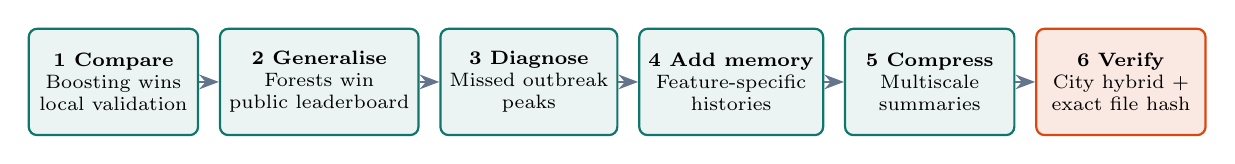
\begin{tikzpicture}[
  node distance=0.25cm,
  stepbox/.style={rectangle,rounded corners=3pt,draw=teal,fill=teal!8,thick,minimum width=2.15cm,minimum height=1.35cm,align=center,font=\scriptsize},
  arr/.style={-{Stealth[length=2.5mm]},thick,slate}]
\node[stepbox] (a) {\textbf{1 Compare}\\Boosting wins\\local validation};
\node[stepbox,right=of a] (b) {\textbf{2 Generalise}\\Forests win\\public leaderboard };
\node[stepbox,right=of b] (c) {\textbf{3 Diagnose}\\Missed outbreak\\peaks};
\node[stepbox,right=of c] (d) {\textbf{4 Add memory}\\Feature-specific\\histories};
\node[stepbox,right=of d] (e) {\textbf{5 Compress}\\Multiscale\\summaries};
\node[stepbox,right=of e,fill=ember!12,draw=ember] (f) {\textbf{6 Verify}\\City hybrid +\\exact file hash};
\foreach \x/\y in {a/b,b/c,c/d,d/e,e/f} \draw[arr] (\x)--(\y);
\end{tikzpicture}
\caption{The experiment map. A disappointing result or visible failure mode triggered each next experiment.}
\label{fig:map}
\end{figure}

%--------------------------------------------------------------------
\section{Data}
%--------------------------------------------------------------------
\subsection{Loading and splitting}
We load the three CSV files with \texttt{pandas}: features, labels, and the test features. Training features and labels are joined on the key (\texttt{city}, \texttt{year}, \texttt{weekofyear}) with a one-to-one check, giving a table with $1456$ rows. The inputs $X$ are the weekly climate columns and the target $y$ is \texttt{total\_cases}. The test keys are verified to match the submission template exactly, so predictions can be written in the required order.

\begin{table}[H]
\centering
\caption{Dataset overview.}
\label{tab:data}
\begin{tabular}{lrr}
\toprule
& \textbf{San Juan (SJ)} & \textbf{Iquitos (IQ)}\\
\midrule
Training weeks & 936 & 520\\
Test weeks (public) & 260 & 156\\
Training period & 1990--2008 & 2000--2010\\
Median weekly cases & 19 & 5\\
Mean weekly cases & 34.2 & 7.6\\
Maximum weekly cases & 461 & 116\\
\bottomrule
\end{tabular}
\end{table}

The $24$ test columns comprise three key columns, the date, four NDVI indices, and $16$ weather series from stations and reanalysis. Tree models use NDVI summaries as well as weather. The final MLP expands only the $16$ consistently defined weather series, plus calendar phase: NDVI has substantially more missingness and did not provide stable lag-window evidence. This is why ``24 columns'' becomes $16$ temporally engineered signals rather than $24$ lagged variables.

\subsection{Two cities, two target distributions}
Figure~\ref{fig:target} shows the weekly case series and their distributions. San Juan has rare, very large outbreaks (maximum $461$, median $19$), while Iquitos has smaller counts with many near-zero weeks (maximum $116$, median $5$). Both distributions are strongly right-skewed.

\begin{figure}[H]
\centering
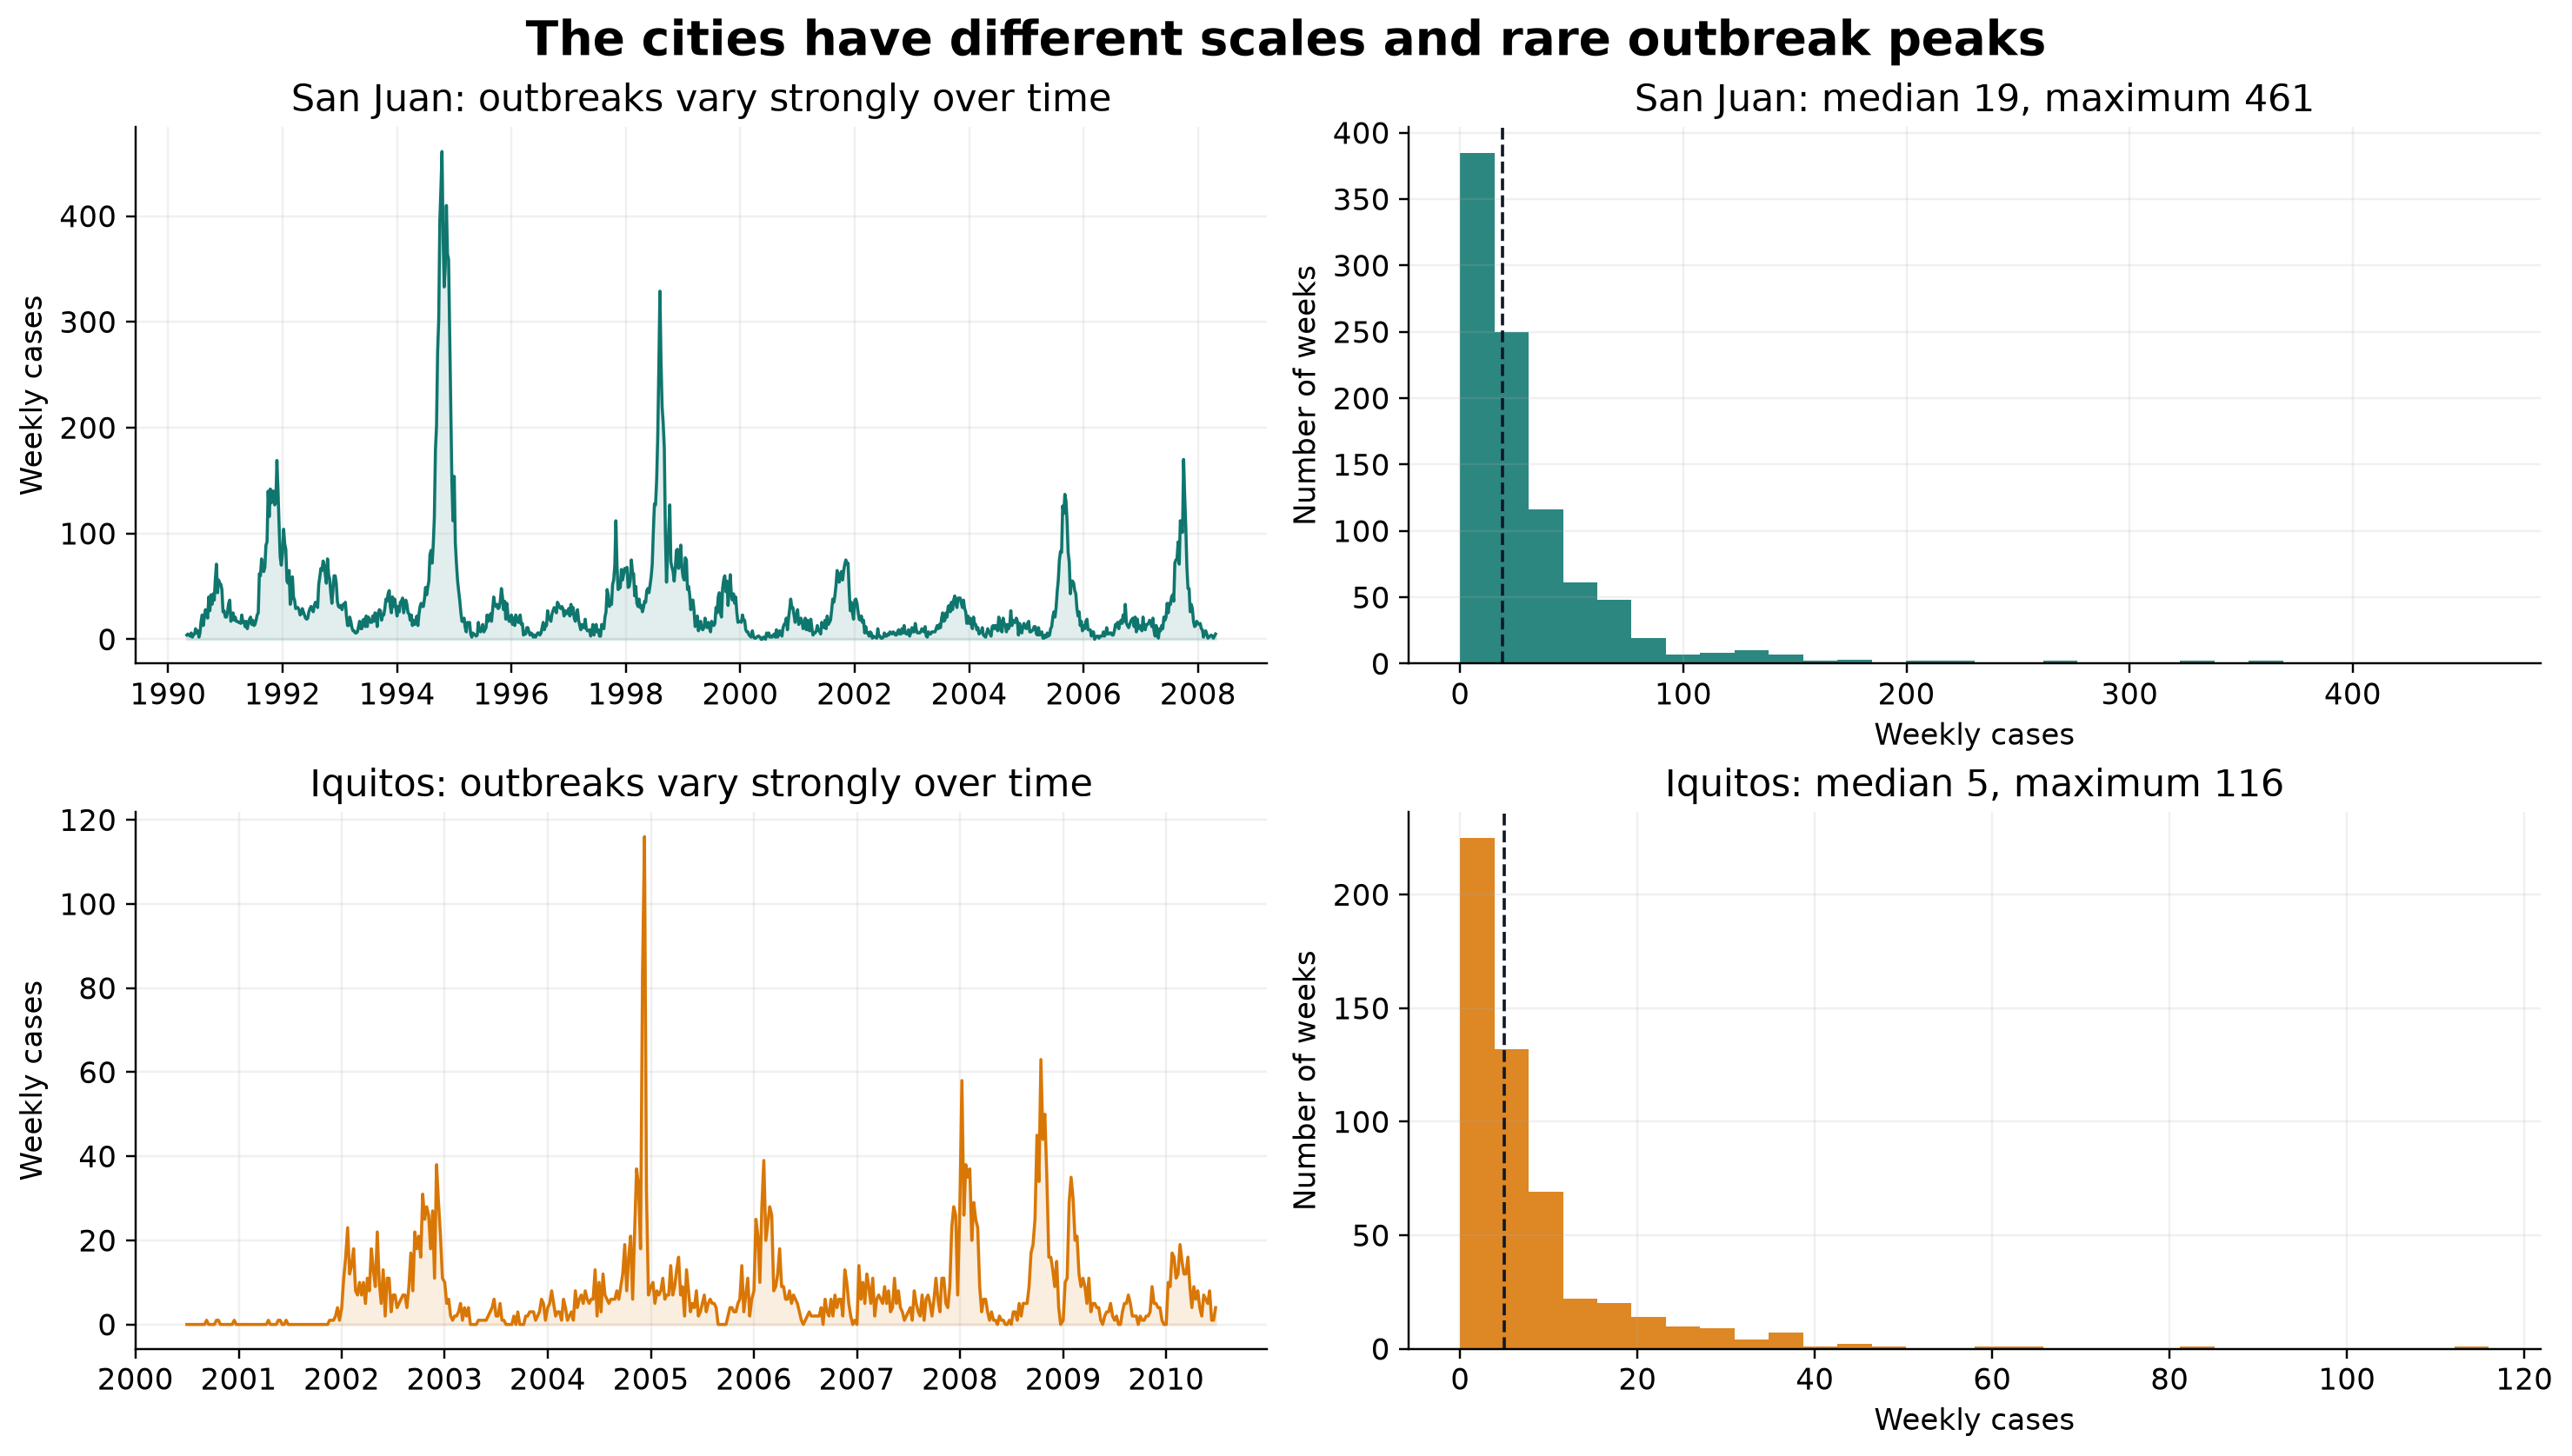
\includegraphics[width=0.95\linewidth]{figures/01_target_scale_and_outbreaks.png}
\caption{Weekly cases per city (left) and their distributions with the median marked (right). The scales differ by roughly a factor of four and both are dominated by rare peaks.}
\label{fig:target}
\end{figure}

\key{Decision.} The cities differ in scale, climate and outbreak behaviour, so we train and tune a \emph{separate model for each city}. Because the metric is absolute error and outbreaks are rare, we also report error separately on outbreak weeks (weeks above a city-specific high-case threshold) in addition to the mean.

%--------------------------------------------------------------------
\section{Exploratory analysis}
%--------------------------------------------------------------------
\subsection{Seasonality helps but does not decide}
Figure~\ref{fig:season} plots the mean, median and interquartile range of cases per calendar week. San Juan peaks in the second half of the year (highest mean around week~40) and Iquitos shows a late-year peak (around week~50) with an additional early-year bump. However, the interquartile bands are wide: the same week of the year can have very different outcomes in different years.

\begin{figure}[H]
\centering
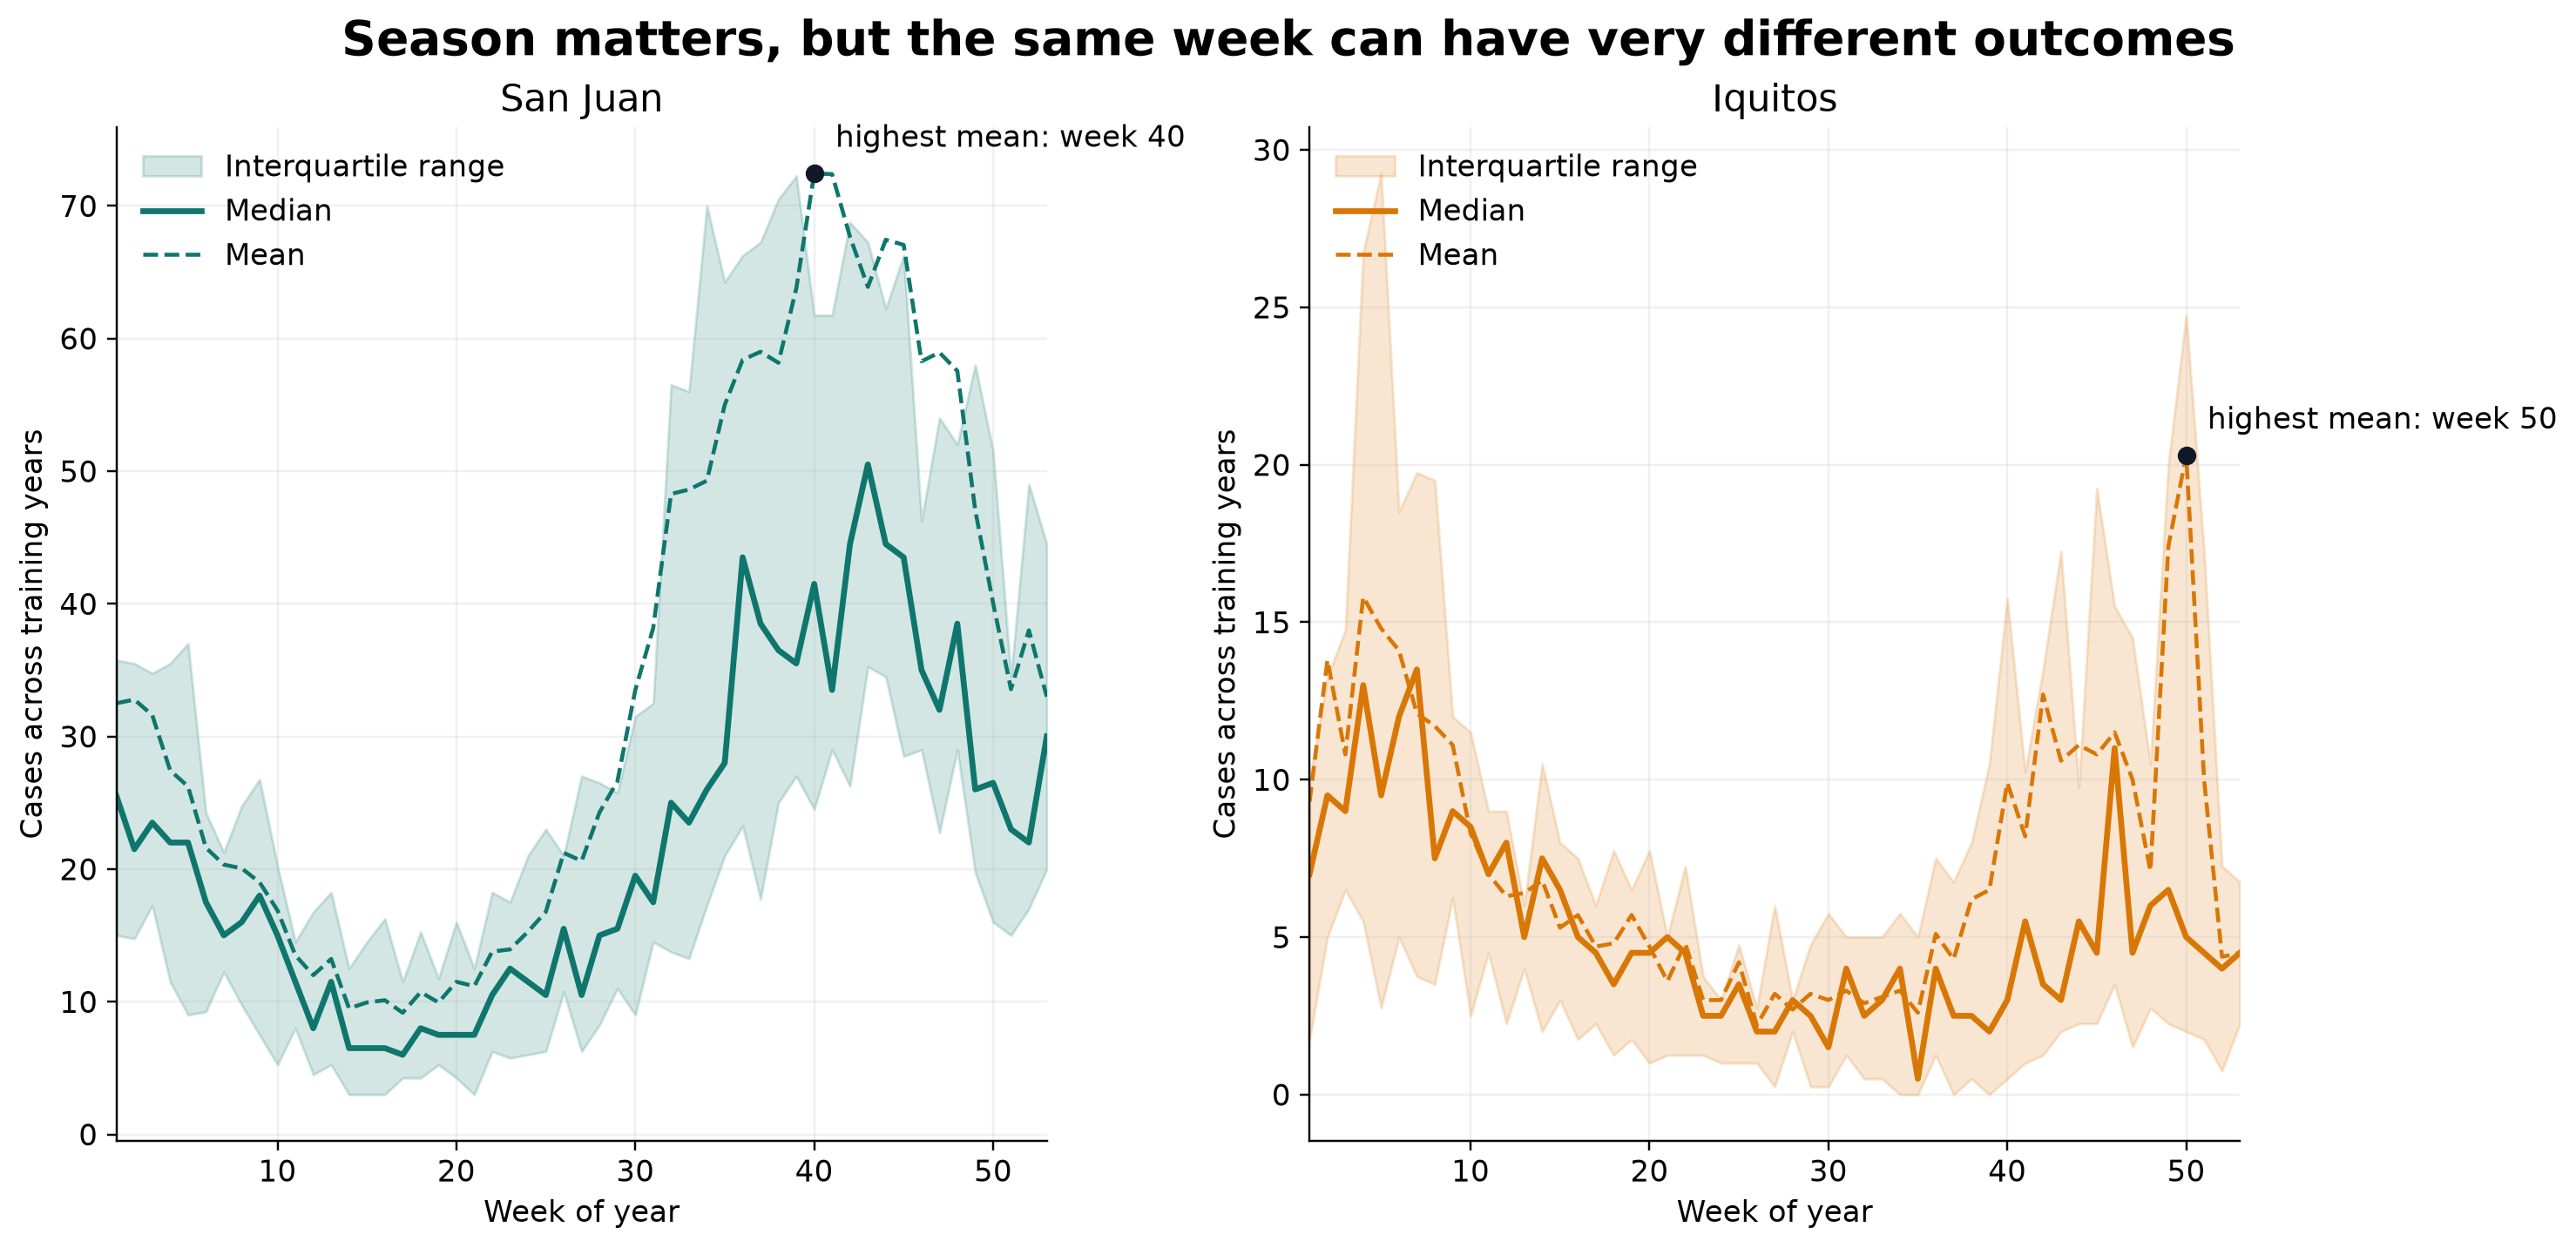
\includegraphics[width=0.95\linewidth]{figures/02_seasonal_case_pattern.png}
\caption{Cases by calendar week across training years. The seasonal signal is real, but the wide band shows that calendar week alone does not determine the count.}
\label{fig:season}
\end{figure}

\key{Decision.} The model needs the \emph{calendar phase} (as continuous sine/cosine terms so that week~52 and week~1 are neighbours) \emph{and} recent climate conditions.

\subsection{Missing values}
Missing values are rare but not negligible: the training features contain $548$ missing cells. Figure~\ref{fig:missing} lists the variables missing in at least $1\%$ of training weeks. The northeast NDVI index in San Juan is the worst case (about $20\%$), followed by several Iquitos station temperature variables (about $7\%$).

\begin{figure}[H]
\centering
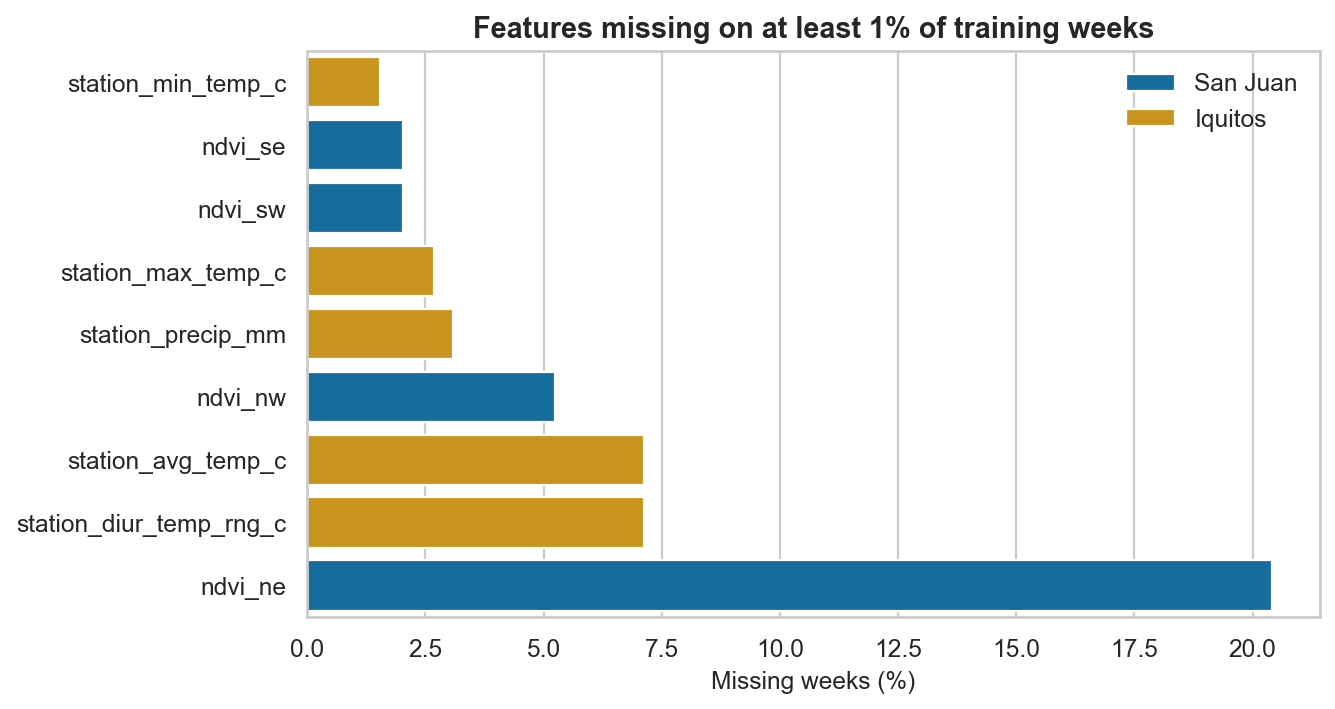
\includegraphics[width=0.9\linewidth]{figures/03_missingness.png}
\caption{Share of training weeks with a missing value, by variable and city.}
\label{fig:missing}
\end{figure}

\subsection{Case counts have memory; climate memory is variable-specific}
Figure~\ref{fig:memory} illustrates two
important characteristics of dengue incidence
and climate history.

First, the autocorrelation of weekly dengue cases
decreases gradually over approximately 15--20 weeks,
with stronger temporal persistence in San Juan
than in Iquitos.

This suggests that dengue incidence is not
independent across weeks and motivates
investigating historical climate information.

Second, different weather variables appear
to require different history lengths.

To investigate this, we considered candidate
history windows ranging from 3 to 51 weeks
for each weather variable and city.

For a variable $v$, a window of length $L$
contains consecutive observations:

\begin{equation}
\mathbf{x}_{t}^{(v,L)}
=
[x_{t-L+1}^{(v)}, \ldots, x_t^{(v)}].
\end{equation}

A decision-tree screening procedure was used
to compare candidate window lengths.

However, the original screening employed
ordinary ten-fold validation rather than
strictly chronological folds. Therefore,
the selected lengths should be interpreted
as exploratory feature-engineering choices,
not unbiased estimates of optimal
forecasting horizons.

The results suggest that useful climate
history differs across variables and cities.

For example, the selected relative-humidity
history was 34 weeks for San Juan but only
7 weeks for Iquitos.

These observations motivated the
city-specific historical representations
investigated in Section~6.3.
\begin{figure}[H]
\centering
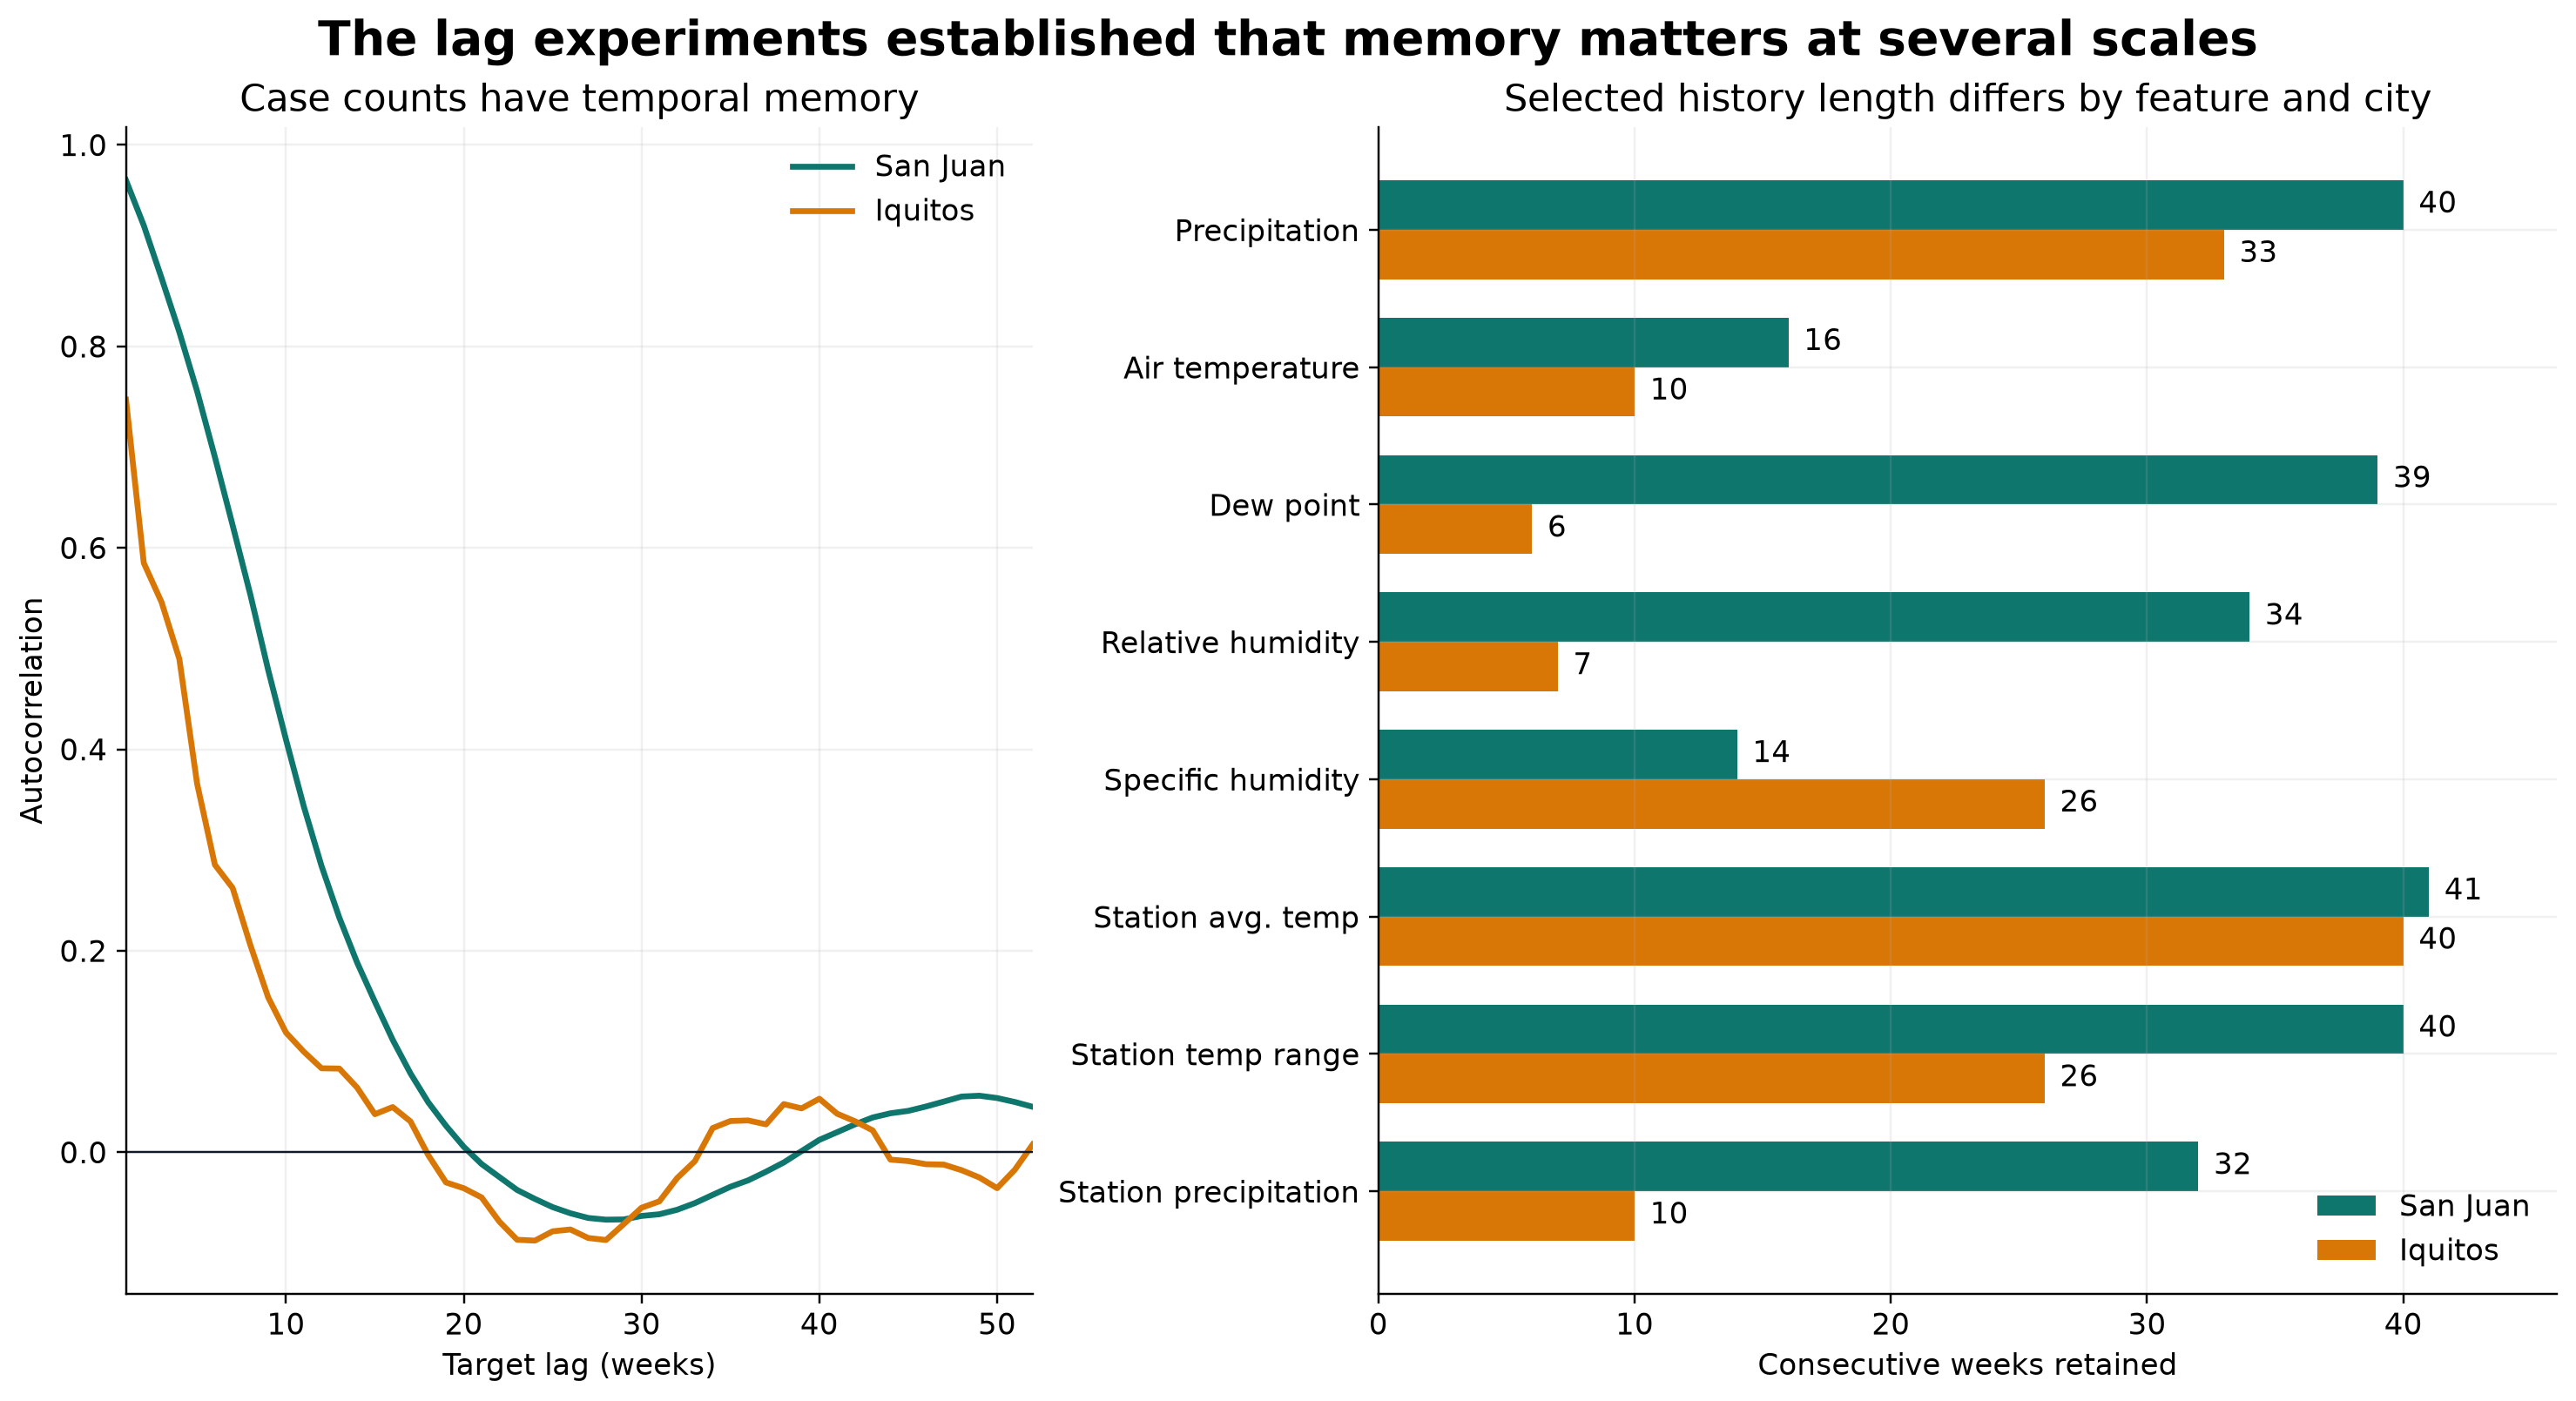
\includegraphics[width=\linewidth]{figures/03_temporal_memory_patterns.png}
\caption{Left: autocorrelation of cases. Right: history length (number of consecutive weeks retained) chosen by the screening step, per weather variable and city.}
\label{fig:memory}
\end{figure}

\textbf{Caveat.} The original ten-fold procedure used for this screen was not fully forecasting-safe, so exact values such as $39$ versus $40$ weeks should not be read as biological constants. We use the screen only as evidence that memory is long, variable-specific and city-specific.

%--------------------------------------------------------------------
\section{Preprocessing and feature engineering}
%--------------------------------------------------------------------
Every transformation below is motivated by one of the findings above. Test-time features use only climate observations available at the model's recorded history endpoint. For exact experimental compatibility, the reproduction notebook also retains the original two-row alignment and circular context used to construct the earliest training windows; we document this implementation quirk rather than silently changing the submitted model.

\begin{table}[H]
\centering
\caption{Preprocessing steps and the reason for each.}
\label{tab:prep}
\small
\begin{tabular}{>{\raggedright\arraybackslash}p{3.2cm}>{\raggedright\arraybackslash}p{5.3cm}>{\raggedright\arraybackslash}p{6cm}}
\toprule
\textbf{Step} & \textbf{What we do} & \textbf{Why}\\
\midrule
Missing values, forests & Median imputer fitted on the training fold & The median is robust and fold-fitting avoids leakage\\
Missing values, boosting & XGBoost/CatBoost native missing-value routing & Each split learns a default direction for unavailable values; no global fill value is required\\
Missing values, MLP & Linear interpolation in time order & Weather is smooth over a week; interpolation avoids breaking history windows\\
Scaling (tree models) & None: raw units are retained & Split order is unchanged by monotone rescaling; scaling adds no benefit to XGBoost, CatBoost, Random Forest or Extra Trees\\
Scaling (MLP) & $z$-scores of weather columns using San Juan statistics; week of year min--max scaled & Variables are in different units; networks are scale-sensitive\\
Season & $\sin/\cos$ of $2\pi\,\mathrm{week}/52$ (and $4\pi$ for tree models, four harmonics) & Smooth, continuous yearly cycle across the new-year boundary\\
Target & Predict cases directly with an absolute-error loss; Iquitos trees use $\log(1{+}y)$ & MAE is the competition metric; log stabilises Iquitos' small counts for forests\\
Per-city models & One model and one set of hyper-parameters per city & Different scales, histories and regimes (Section~3)\\
\bottomrule
\end{tabular}
\end{table}

\subsection{Exactly what XGBoost and CatBoost received}
The boosting comparison used the same information as the confirmed forest, so it was a model comparison rather than a different-feature comparison. We sorted each city chronologically, removed identifiers that should not drive prediction (\texttt{city}, date and target), and removed calendar year for the boosting candidates because extrapolating a numerical year trend into a three- or five-year test block was unsafe. All remaining inputs were numeric; CatBoost was not given categorical columns.

For each weekly row, the design matrix contained current climate and NDVI measurements, eight Fourier coordinates (four annual harmonics), NDVI mean and spatial spread, two temperature ranges, a temperature--humidity interaction, nine weather variables at lags $1,2,4,8,12,16$, and past-only means over $2,4,8,12,16$ weeks. Rolling means were shifted by one week. Consequently, ``past mean 4'' at week $t$ used $t-1$ through $t-4$, never the current value and never a future value. Previous dengue counts were excluded because true case labels are unavailable throughout the hidden horizon.

\begin{table}[H]
\centering
\caption{Preprocessing and regularisation in the first model comparison.}
\label{tab:boostprep}
\small
\begin{tabular}{>{\raggedright\arraybackslash}p{2.5cm}>{\raggedright\arraybackslash}p{4.8cm}>{\raggedright\arraybackslash}p{6.5cm}}
\toprule
\textbf{Model} & \textbf{Input handling} & \textbf{Main controls used in the experiment}\\
\midrule
XGBoost & Same engineered numeric matrix; missing values handled by the learner; no standardisation & $500$ boosting rounds, learning rate $0.03$, depth $2$ or $3$, minimum child weight $10$, row subsampling $0.85$, feature subsampling $0.8$, L1 $0.1$, L2 $10$; MAE and Poisson objectives tested\\
CatBoost & Same engineered numeric matrix; native missing-value routing; no categorical features and no standardisation & $500$ iterations, learning rate $0.03$, depth $4$ or $6$, L2 leaf penalty $10$, Bernoulli subsampling $0.85$, random strength $0.5$; MAE and Poisson losses tested\\
Random Forest / Extra Trees & Fold-fitted median imputation; no standardisation & $500$ trees and at least five samples per leaf; city-specific target/criterion described in Section~\ref{sec:foreststage}\\
\bottomrule
\end{tabular}
\end{table}

The boosting targets were the observed case counts: Poisson candidates enforced a count-compatible objective and MAE candidates matched the leaderboard loss. We did not normalize the target. Only the Iquitos forest applied $\log(1+y)$ and transformed its predictions back with $\exp(\hat z)-1$. Every learned imputation rule and every fitted model used only the earlier part of each chronological fold.

\subsection{Three feature sets}
\paragraph{(A) Tree features.} For each week: current climate; four annual Fourier harmonics (eight seasonal coordinates); NDVI mean and spread over the four locations; temperature ranges; a temperature $\times$ humidity interaction; climate at lags $1,2,4,8,12,16$; and trailing means over $2,4,8,12,16$ weeks (computed with a one-week shift so the current row cannot leak into its own summary).

\paragraph{(B) Raw lag windows.} For each weather variable $v$ and city $c$ we keep a window of $L_{v,c}$ \emph{consecutive} past values (not a single lag). Concatenating all windows gives one flat vector: $461$ inputs for San Juan and $380$ for Iquitos. A $40$-week window keeps all $40$ consecutive values, not only the value at lag $40$.

\paragraph{(C) Multiscale summaries.} For each of the $16$ weather variables we compute $11$ statistics from the previous $52$ weeks, and add four seasonal terms:
\begin{enumerate}[label=\arabic*.]
  \item the current (latest) value;
  \item means over $2,4,8,13,26,52$ weeks (climate level at several timescales);
  \item standard deviations over $4$ and $13$ weeks (recent and medium-term variability);
  \item the $4$-week mean minus the $13$-week mean (short-term conditions relative to baseline);
  \item a $13$-week trend, $\bigl(x_t-x_{t-12}\bigr)/12$ (direction and rate of change);
  \item $\sin,\cos$ of $2\pi\,\mathrm{week}/52$ and of $4\pi\,\mathrm{week}/52$ (cyclic seasonality).
\end{enumerate}
The size is $16\times 11+4=\mathbf{180}$ inputs. The final San Juan model uses these $180$ inputs; the final Iquitos model retains its $380$ raw-lag inputs.

%--------------------------------------------------------------------
\section{Validation protocol and metric}
%--------------------------------------------------------------------
\subsection{Why chronological validation}
A random split places neighbouring outbreak weeks on both sides of the split. The model can then ``interpolate'' an outbreak from adjacent weeks that would never be available in a real forecast, giving an optimistic score. The public test period lies strictly after the training period, so validation must have the same direction.

We use \key{expanding-window folds}: fold $k$ trains on all weeks before a cut point and is evaluated on the next $52$ weeks (Figure~\ref{fig:cv}). All preprocessing that learns from data (imputation, scaling, any projection) is fitted inside the training window of each fold.

\begin{figure}[H]
\centering
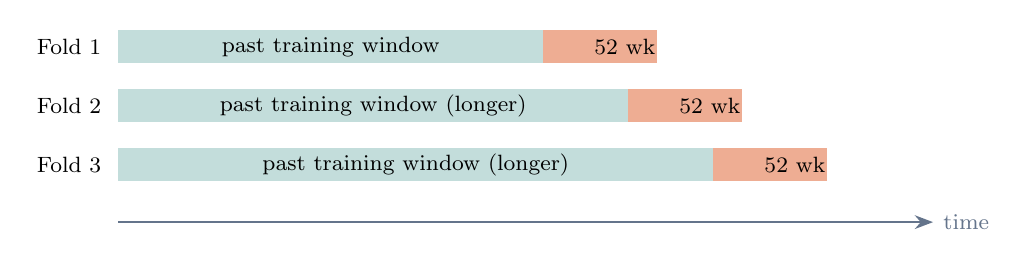
\begin{tikzpicture}[x=0.9cm,y=0.75cm,font=\footnotesize]
\foreach \i/\n in {0/1,1/2,2/3}{
  \fill[teal!25] (0,-\i) rectangle (6+\i*1.2,-\i+0.55);
  \fill[ember!45] (6+\i*1.2,-\i) rectangle (8.4+\i*1.2-0.8,-\i+0.55);
  \node[anchor=east] at (-0.1,-\i+0.27) {Fold \n};
}
\node at (3,0.27) {past training window};
\node at (7.15,0.27) {52 wk};
\node at (3.6,-0.73) {past training window (longer)};
\node at (8.35,-0.73) {52 wk};
\node at (4.2,-1.73) {past training window (longer)};
\node at (9.55,-1.73) {52 wk};
\draw[-{Stealth},thick,slate] (0,-2.7) -- (11.5,-2.7) node[right] {time};
\end{tikzpicture}
\caption{Expanding folds: the model never sees data later than the period it is scored on.}
\label{fig:cv}
\end{figure}

\subsection{Information availability and forecasting assumptions}

Let $t$ denote the target week and
$\mathcal{I}_t$ denote the information
available when the prediction is issued.

A valid prospective forecasting pipeline
must construct every predictor from
information available at that time:

\begin{equation}
\hat{y}_t = f(\mathcal{I}_t).
\end{equation}

In the DengAI benchmark, weather features
are provided for the prediction period.
Our competition experiments use these
supplied climate measurements.

However, access to climate observations
for the target week is not equivalent to
having those measurements available before
the week begins.

Therefore, the benchmark performance
should be interpreted as climate-conditioned
case prediction unless the operational
availability of the weather measurements
is independently established.

A prospective forecasting evaluation would
require a defined forecast issuance time and
appropriate historical observations or
weather forecasts available at that time.

\subsection{Metric}
We use MAE because it is the competition metric and is less dominated by single extreme weeks than squared error. We report three numbers per configuration: the \emph{mean} MAE across folds, the \emph{worst-fold} MAE (stability), and the \emph{outbreak-week} MAE (the weeks that matter most for public health). The same folds are used for every model so that differences measure the model and not the split.
\begin{equation}
\mathrm{MAE}_{\mathrm{outbreak},c}
=
\frac{1}{|\mathcal{O}_c|}
\sum_{t\in\mathcal{O}_c}
|y_t-\hat{y}_t|,
\end{equation}
where $\mathcal{O}_c$ denotes the set of
validation weeks classified as outbreaks
for city $c$.

The outbreak threshold is defined using
the training data and held fixed when
evaluating the corresponding validation fold.
\subsection{Baselines}
Figure~\ref{fig:baseline} compares a historical-mean predictor, a week-of-year climatology (the median or mean for that calendar week) and a tuned tree ensemble on the same $312$ weeks per city. Climatology is very hard to beat in Iquitos ($6.8$ vs.\ $7.1$ for the trees), whereas in San Juan climate features cut the error from $25.1$ to $15.7$. Figure~\ref{fig:valforecast} shows why San Juan is difficult: climatology predicts a smooth seasonal hump every year, while actual outbreaks are irregular.

\begin{figure}[H]
\centering
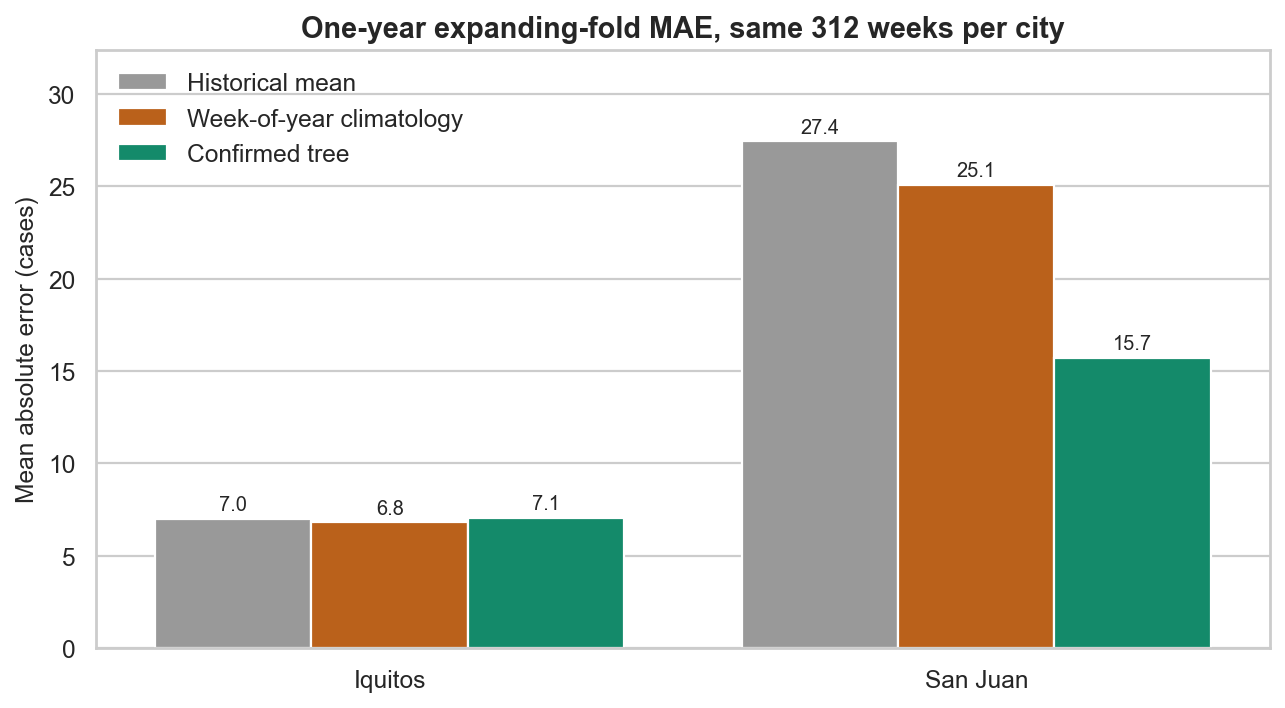
\includegraphics[width=0.72\linewidth]{figures/06_baseline_comparison.png}
\caption{One-year expanding-fold MAE on identical $312$ validation weeks per city.}
\label{fig:baseline}
\end{figure}

\begin{figure}[H]
\centering
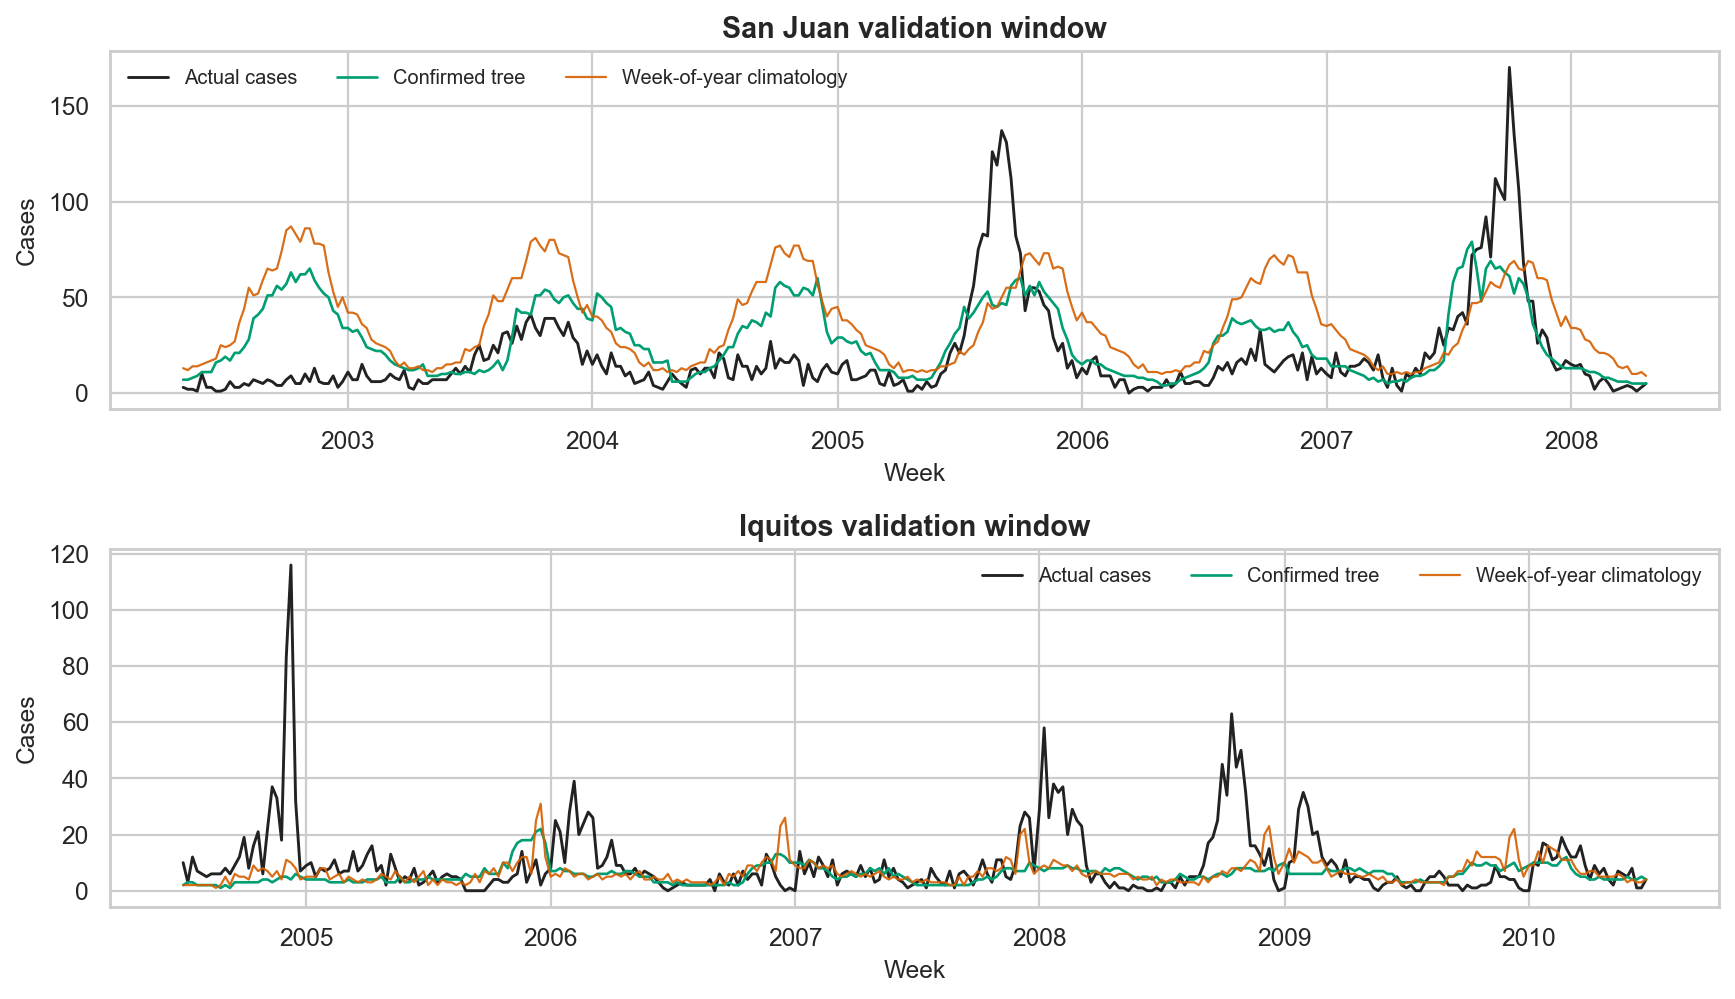
\includegraphics[width=\linewidth]{figures/05_validation_forecasts.png}
\caption{Validation windows: actual cases, a confirmed tree model, and week-of-year climatology. Peaks of the largest outbreaks are underestimated.}
\label{fig:valforecast}
\end{figure}

%--------------------------------------------------------------------
\section{Models and experiments}
%--------------------------------------------------------------------
\subsection{Stage 0: the first ranking reversal}
Our first serious comparison used XGBoost \cite{xgboost}, CatBoost \cite{catboost} and a Random-Forest family baseline \cite{rf}. The early training and validation runs favoured the boosted learners: sequentially correcting residuals let them fit small irregularities that a bagged forest averaged away. The archived controlled experiment confirms the local part of that observation. It selected a $20\%$ XGBoost contribution for Iquitos and a $40\%$ CatBoost contribution for San Juan, and both the four-fold selection score and the six-fold report score improved over the forest system (Table~\ref{tab:rankingflip}).

\begin{table}[H]
\centering
\caption{The local ranking that did not survive the hidden period. The boosted row is a city-specific blend, not a claim that one boosted model won both cities.}
\label{tab:rankingflip}
\small
\begin{tabular}{>{\raggedright\arraybackslash}p{3.5cm}ccc}
\toprule
\textbf{Candidate} & \textbf{4-fold local MAE} & \textbf{6-fold local MAE} & \textbf{Hidden-test outcome}\\
\midrule
City-specific forest & 10.091 & 11.393 & \textbf{22.5; retained}\\
Selected boosted blend & \textbf{9.788} & \textbf{11.061} & Worse than forest; rejected\\
\bottomrule
\end{tabular}
\end{table}

The leaderboard reversed the local ranking: the simpler forest submission generalized better. We cannot prove whether this was ordinary model-selection overfitting, temporal distribution shift, or both, because the hidden labels are unavailable. The important engineering conclusion was operational: a small local MAE advantage on a few dependent time folds was not enough evidence to trust a more adaptive model. This changed our selection rule from ``take the lowest validation mean'' to ``also inspect fold variance, peak amplitude and behaviour on a test-length horizon.''

\subsection{Stage 1: lower-variance forest ensembles (public leaderboard MAE $22.5$)}
\label{sec:foreststage}
We next focused on variance. Random Forest fits trees to bootstrap samples and random feature subsets. Extra Trees goes further: for candidate features it randomizes the split thresholds before choosing a split. This extra randomisation makes the individual trees less similar. If $T$ trees have variance $\sigma^2$ and average pairwise correlation $\rho$, the variance of their average is approximately
\begin{equation}
\operatorname{Var}(\bar f) = \frac{\sigma^2}{T}\left[1+(T-1)\rho\right].
\end{equation}
With $T=500$, reducing correlation $\rho$ is at least as important as adding more trees. Extra Trees can therefore reduce ensemble variance, although excessive randomisation can increase bias. We controlled the other major source of variance by requiring at least five training examples in every leaf.

The selected city-specific system used the causal tree features of set (A):
\begin{itemize}
  \item San Juan: $500$-tree Extra Trees \cite{extratrees} with Poisson splitting;
  \item Iquitos: $500$-tree Random Forest trained on $\log(1+y)$;
  \item minimum five samples per leaf to avoid very specific rules.
\end{itemize}

\paragraph{How the ensemble prediction is formed.} This is not a vague vote among model names. Within one city, every tree produces a real-valued case forecast and the forest averages the $500$ outputs:
\begin{equation}
\hat y_{c,t}=\frac{1}{500}\sum_{b=1}^{500} f_{c,b}(x_{c,t}).
\end{equation}
For Iquitos the average is formed on the $\log(1+y)$ scale and then inverted; for San Juan the trees predict the count directly with the Poisson split criterion. Predictions are clipped at zero and rounded to an integer. We do \emph{not} average San Juan and Iquitos models together: the San Juan model predicts San Juan rows, the Iquitos model predicts Iquitos rows, and the two blocks are concatenated in the official submission order.

We also tested explicit forest--boosting blends,
\begin{equation}
\hat y=(1-w)\hat y_{\mathrm{forest}}+w\hat y_{\mathrm{boost}},
\end{equation}
with $w\in\{0,0.1,\ldots,1.0\}$. Local validation selected $w=0.2$ with XGBoost for Iquitos and $w=0.4$ with CatBoost for San Juan. Those blends are the second row of Table~\ref{tab:rankingflip}; because their public leaderboard result was worse, they were experiments, not the submitted $22.5$ tree system.
Trees capture non-linear thresholds (``warm \emph{and} humid after several wet weeks''), lags express delayed effects, rolling means express accumulated exposure, and Fourier terms express season. This reduced public leaderboard MAE from $26.7$ to $22.5$. But the validation forecast in Figure~\ref{fig:valforecast} exposed the next problem: the forest followed the seasonal level while repeatedly cutting off the largest peaks.

\subsubsection*{Residual Analysis \& Feature Engineering}
We inspected the largest absolute residuals week by week. Several outbreak weeks had a sudden increase in cases even though the weather in that same row was not unusually extreme. The model had learned an overly instantaneous mapping---``this week's weather predicts this week's cases''---while the real process includes mosquito development, viral incubation and reporting delays. A rainfall or humidity episode can therefore matter weeks before the observed case peak.

\begin{figure}[H]
\centering
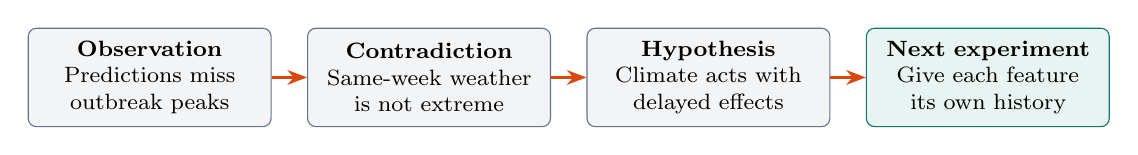
\begin{tikzpicture}[
  node distance=0.45cm,
  pbox/.style={rectangle,rounded corners=3pt,draw=slate,fill=slate!8,text width=2.85cm,minimum height=1.25cm,align=center,font=\footnotesize},
  arr/.style={-{Stealth[length=2.5mm]},thick,ember}]
\node[pbox] (o) {\textbf{Observation}\\Predictions miss outbreak peaks};
\node[pbox,right=of o] (c) {\textbf{Contradiction}\\Same-week weather is not extreme};
\node[pbox,right=of c] (h) {\textbf{Hypothesis}\\Climate acts with delayed effects};
\node[pbox,right=of h,draw=teal,fill=teal!9] (e) {\textbf{Next experiment}\\Give each feature its own history};
\foreach \x/\y in {o/c,c/h,h/e} \draw[arr] (\x)--(\y);
\end{tikzpicture}
\caption{Error analysis converted a visible failure mode into the lag-window experiment.}
\label{fig:errorlogic}
\end{figure}

This was the project's main pivot. We stopped asking only ``which learner wins?'' and asked ``what information is missing from the input?'' The answer was not one universal lag for all variables, but a city- and feature-specific history.
\subsection{Stage 2: an MLP with lagged inputs (public leaderboard MAE $19.3\rightarrow18.8$)}
\paragraph{Lagged climate associations.}

We first examined the association between
individual historical climate measurements
and dengue incidence at different temporal lags.

Figure~\ref{fig:lag_heatmap} illustrates
these associations for selected weather variables.
The correlations vary with lag, variable,
and city, motivating further investigation
of historical climate representations.

However, lagged correlation is not equivalent
to predictive performance, and the lag with
the largest correlation does not necessarily
define the optimal history-window length.
\begin{figure}[H]
\centering
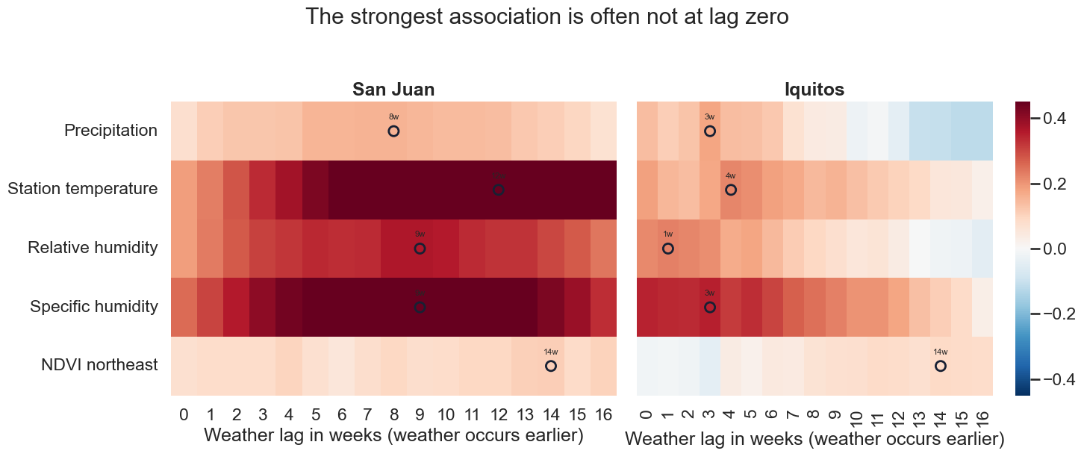
\includegraphics[width=\linewidth]{figures/heatmap_lags.png} %
\caption{Lagged correlations between selected climate
variables and weekly dengue cases in San Juan
and Iquitos. The color scale represents signed
correlation coefficients rather than prediction
MAE. The plot illustrates temporal associations
but does not determine the optimal length of
a predictive history window.}
\label{fig:lag_heatmap}
\end{figure}
A $40$-week choice therefore means all $40$ consecutive values, not only lag $40$.

Candidate history lengths were selected
using a separate decision-tree screening
procedure evaluated by MAE.

The correlation heatmap provides exploratory
motivation but should not be interpreted
as the window-selection objective. For example, relative humidity used $34$ weeks in San Juan and $7$ in Iquitos. Because the original screen used ordinary ten-fold validation and nearby windows were often nearly tied, we treat exact values such as $39$ versus $40$ as engineering choices, not biological constants. The reliable insight was that climate memory is long, variable-specific and city-specific.

We then gave a neural network this structured memory. Concatenating the selected windows produced $461$ inputs for San Juan and $380$ for Iquitos. The network is a three-layer perceptron with SELU activations \cite{selu}, dropout, a linear output and an absolute-error loss, trained with RMSprop and a plateau learning-rate decay. Figure~\ref{fig:arch} shows the two city architectures.

\begin{figure}[H]
\centering
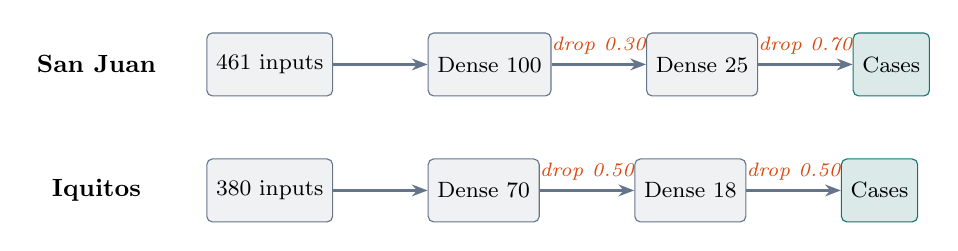
\begin{tikzpicture}[
  box/.style={rectangle,rounded corners=2pt,draw=slate,fill=slate!10,minimum height=0.8cm,font=\footnotesize,align=center},
  drop/.style={font=\scriptsize\itshape,text=ember},
  arr/.style={-{Stealth[length=2mm]},slate,thick}]
\node[font=\small\bfseries] at (-0.6,0.7) {San Juan};
\node[box] (s0) at (1.6,0.7) {461 inputs};
\node[box,right=1.2cm of s0] (s1) {Dense 100};
\node[box,right=1.2cm of s1] (s2) {Dense 25};
\node[box,right=1.2cm of s2,fill=teal!15,draw=teal] (s3) {Cases};
\draw[arr] (s0)--(s1) node[midway,above,drop]{};
\draw[arr] (s1)--(s2) node[midway,above,drop]{drop 0.30};
\draw[arr] (s2)--(s3) node[midway,above,drop]{drop 0.70};
\node[font=\small\bfseries] at (-0.6,-0.9) {Iquitos};
\node[box] (i0) at (1.6,-0.9) {380 inputs};
\node[box,right=1.2cm of i0] (i1) {Dense 70};
\node[box,right=1.2cm of i1] (i2) {Dense 18};
\node[box,right=1.2cm of i2,fill=teal!15,draw=teal] (i3) {Cases};
\draw[arr] (i0)--(i1);
\draw[arr] (i1)--(i2) node[midway,above,drop]{drop 0.50};
\draw[arr] (i2)--(i3) node[midway,above,drop]{drop 0.50};
\end{tikzpicture}
\caption{Raw-history MLPs after temporal tuning. In the multiscale model the input is $180$ for both cities and the San Juan network keeps the same $100\rightarrow25$ hidden layers.}
\label{fig:arch}
\end{figure}

\begin{table}[H]
\centering
\caption{Consecutive history retained by the raw-lag MLP. The entries are window lengths in weeks, not isolated lag positions.}
\label{tab:lagwindows}
\scriptsize
\begin{tabular}{lrr@{\hspace{0.7cm}}lrr}
\toprule
\textbf{Feature} & \textbf{SJ} & \textbf{IQ} & \textbf{Feature} & \textbf{SJ} & \textbf{IQ}\\
\midrule
Precipitation amount & 40 & 33 & Satellite precipitation & 40 & 33\\
Reanalysis air temperature & 16 & 10 & Specific humidity & 14 & 26\\
Reanalysis average temperature & 15 & 4 & Reanalysis diurnal range & 21 & 34\\
Reanalysis dew point & 39 & 6 & Station average temperature & 41 & 40\\
Reanalysis maximum temperature & 12 & 41 & Station diurnal range & 40 & 26\\
Reanalysis minimum temperature & 21 & 40 & Station maximum temperature & 37 & 39\\
Reanalysis precipitation & 30 & 3 & Station minimum temperature & 26 & 25\\
Relative humidity & 34 & 7 & Station precipitation & 32 & 10\\
Week of year & 3 & 3 & & & \\
\bottomrule
\end{tabular}
\end{table}

\paragraph{Tuning.} Under temporal cross-validation, the useful change was a \emph{narrower second hidden layer}, not a deeper network:
\begin{table}[H]
\centering
\caption{Effect of tuning the second hidden layer (mean temporal-CV MAE).}
\begin{tabular}{lccc}
\toprule
 & \textbf{Second layer} & \textbf{Before} & \textbf{After}\\
\midrule
San Juan & $50\rightarrow25$ & 22.02 & 20.64\\
Iquitos & $35\rightarrow18$ & 8.17 & 7.91\\
\bottomrule
\end{tabular}
\end{table}
This gave a public leaderboard MAE of $18.8$ for seed~$42$; averaged over three seeds it is $19.5$, a reminder that a single seed overstates performance.

\paragraph{Remaining problem.} The MLP improved the public leaderboard performance, supporting the time-lag hypothesis, but it created a statistical mismatch. The full dataset has only $1456$ labels, and separate-city training leaves $936$ San Juan labels and $520$ Iquitos labels. Against those sample sizes, the network receives $461$ and $380$ highly correlated coordinates per week. In San Juan the first layer alone has $46{,}100$ input weights. The model must discover simple concepts such as ``recent mean'', ``variability'' and ``trend'' from individual positions, and shifting a wet episode by one week moves its information into many different coordinates. The representation was informative but inefficient.

\paragraph{Why eleven summaries per weather variable.} We did not choose eleven as a magic number. We listed the distinct questions the raw trajectory should answer while remaining small: What is the latest level? What has the average level been over short, monthly, two-month, quarterly, half-year and annual horizons? How volatile has it been recently and over a quarter? Is the recent month above the quarterly baseline? Is the variable rising or falling? These questions become one current value, six means ($2,4,8,13,26,52$ weeks), two standard deviations ($4,13$ weeks), one short-minus-medium contrast, and one $13$-week slope: $1+6+2+1+1=11$. The horizons align with interpretable calendar scales and overlap deliberately, allowing the MLP to compare short- and long-term exposure without seeing all $52$ raw positions.

\subsection{Stage 3: multiscale summaries (public leaderboard MAE $16.6$)}
We therefore replaced raw coordinates with the $180$ summaries of feature set (C) and kept \emph{the same MLP, training procedure and seed}. Under identical chronological folds (three folds, three seeds), summaries lower the mean and worst-fold errors in both cities (Table~\ref{tab:repr}). San Juan improves on mean, worst and outbreak error; Iquitos improves on mean and worst error, while its outbreak MAE rises slightly (from $23.2$ to $23.8$).

\begin{table}[H]
\centering
\caption{Same tuned MLP, chronological validation, three folds and three seeds: raw lag windows vs.\ multiscale summaries (lower is better).}
\label{tab:repr}
\begin{tabular}{llrrr}
\toprule
\textbf{City} & \textbf{Representation} & \textbf{Mean MAE} & \textbf{Worst MAE} & \textbf{Outbreak MAE}\\
\midrule
SJ & Raw lags & 20.635 & 31.942 & 57.095\\
SJ & Multiscale summaries & \textbf{17.726} & \textbf{27.346} & \textbf{55.844}\\
\midrule
IQ & Raw lags & 7.908 & 12.481 & \textbf{23.244}\\
IQ & Multiscale summaries & \textbf{7.588} & \textbf{10.596} & 23.795\\
\bottomrule
\end{tabular}
\end{table}

The multiscale representation reduced the mean
chronological-validation MAE from 20.635 to 17.726
in San Juan and from 7.908 to 7.588 in Iquitos.

On the public leaderboard, the combined MAE
improved from 18.8 to 16.6.
\subsubsection*{Is it compression or just more information?}
If the summaries helped by adding information, then raw lags \emph{plus} summaries should be best. In a two-fold ablation it was the worst (Figure~\ref{fig:ablation}): San Juan MAE was $17.86$ for raw histories, $\mathbf{12.61}$ for summaries and $18.43$ for raw plus summaries.
These results suggest that replacing highly
correlated raw lag coordinates with compact
multiscale summaries provides a more useful
inductive bias for the MLP.

However, the experiment does not isolate
the effects of dimensionality reduction,
optimization, and regularization.

\begin{figure}[H]
\centering
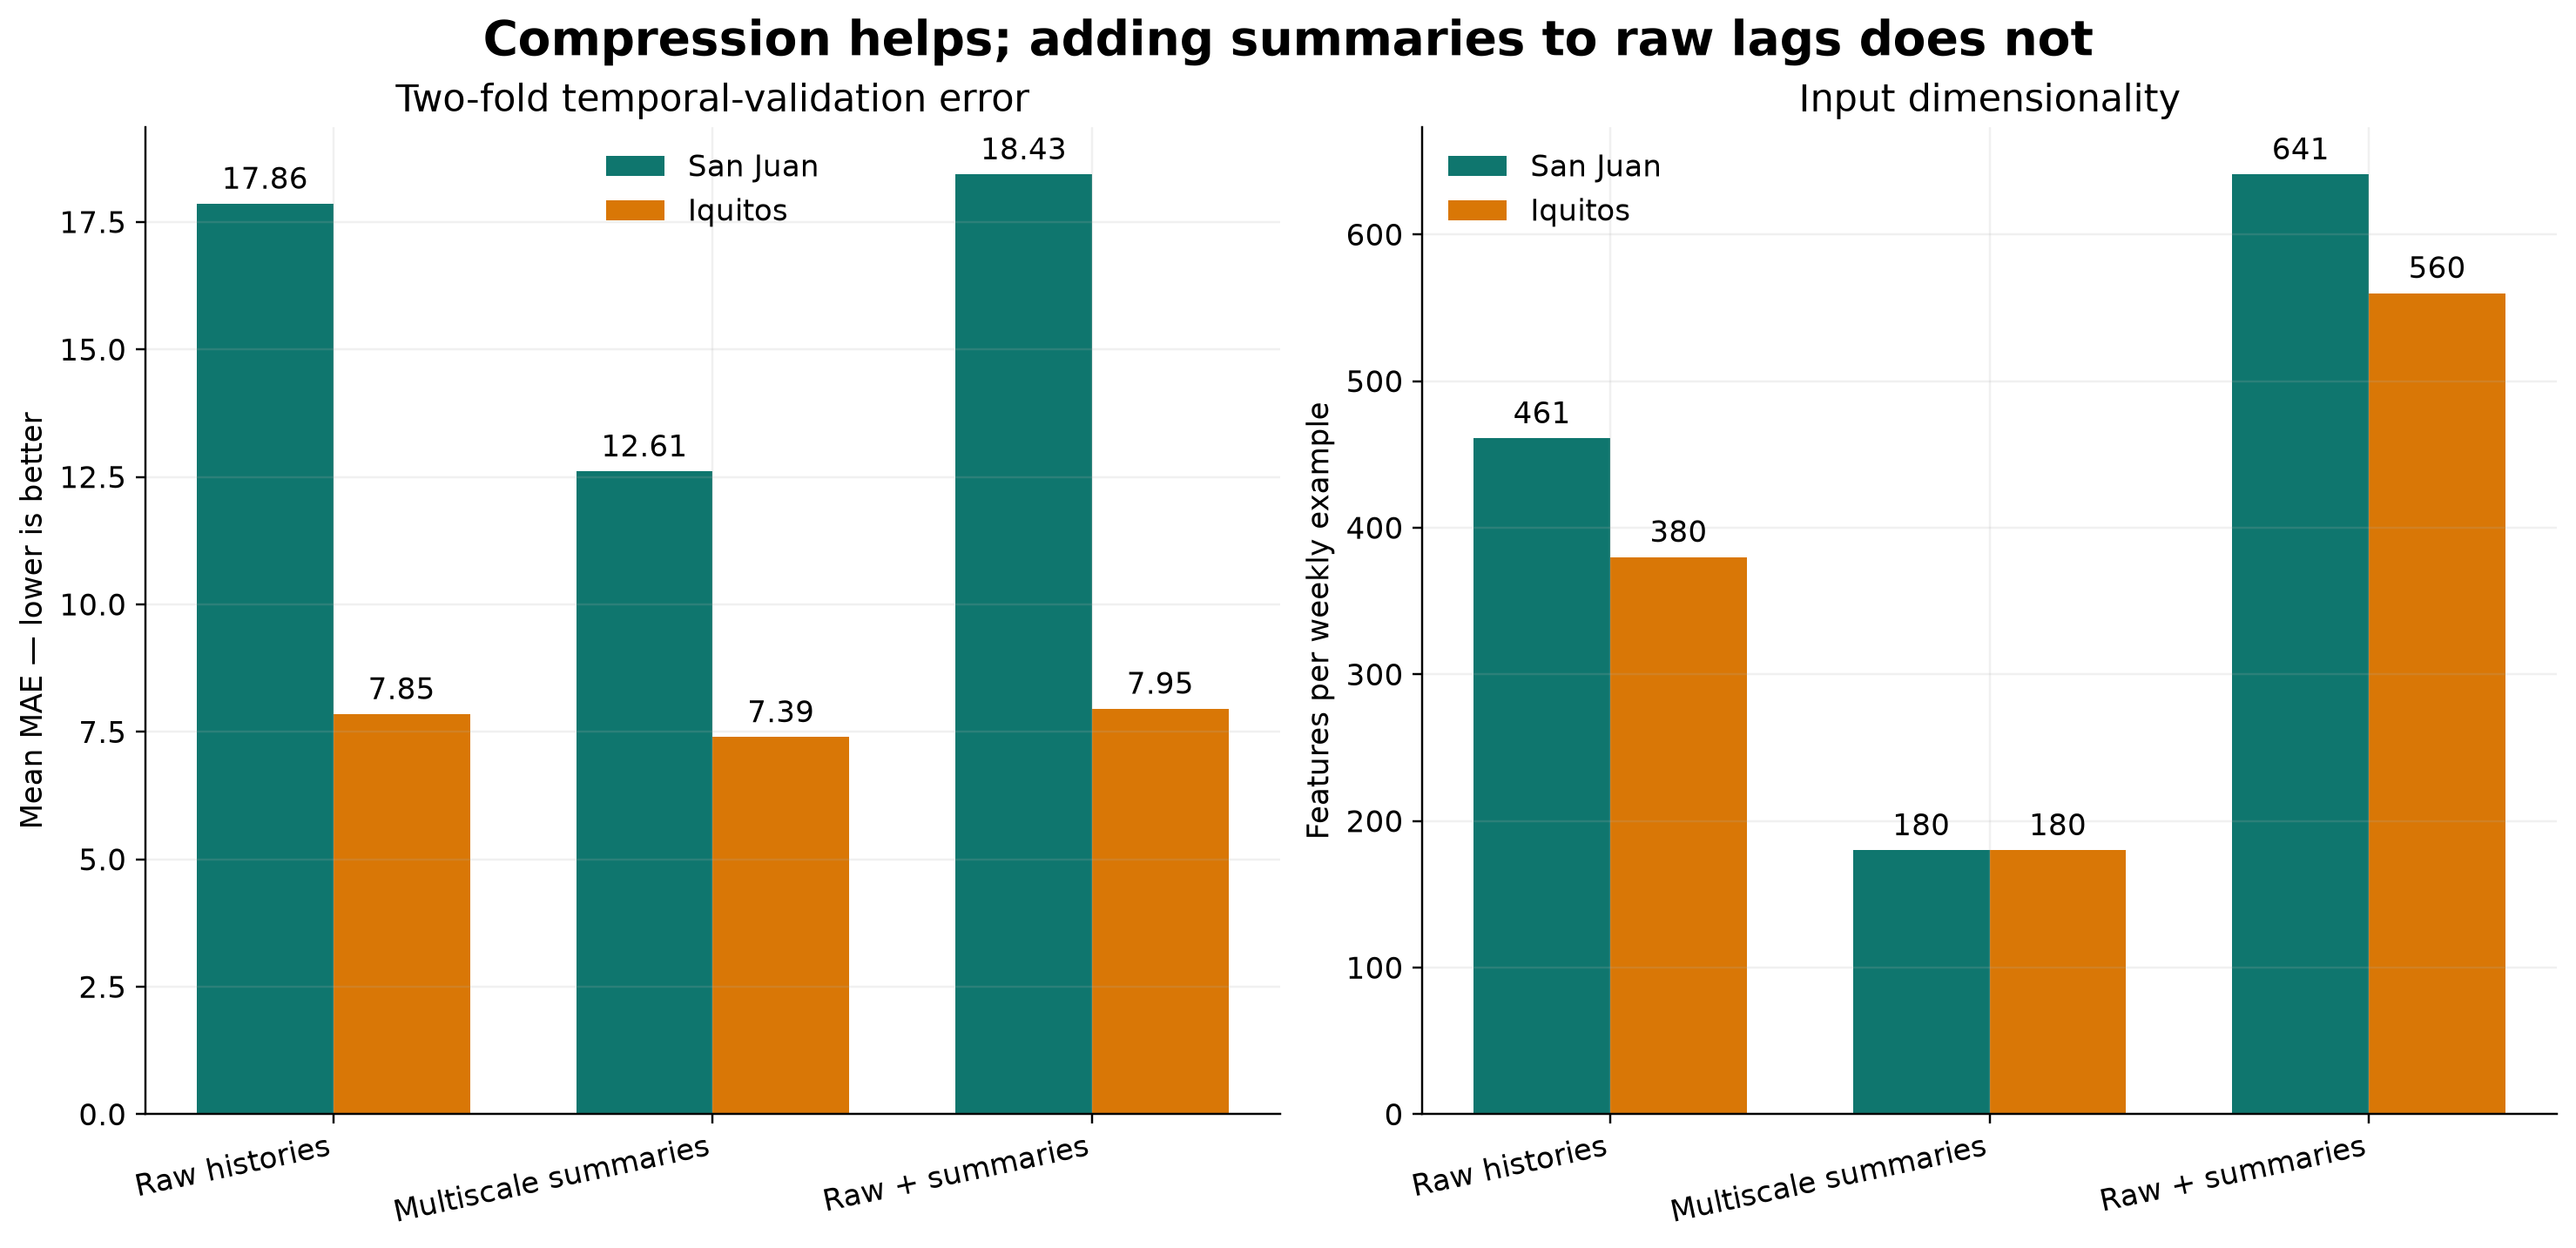
\includegraphics[width=\linewidth]{figures/04_representation_ablation.png}
\caption{Left: two-fold temporal-validation MAE for three input representations. Right: number of inputs per weekly example. Compression helps; adding summaries to raw lags does not.}
\label{fig:ablation}
\end{figure}

\subsection{Stage 4: select, round and reproduce the exact $15.9832$ submission}
\label{sec:finalrecipe}
The restored scored file resolved an important provenance question. Its recorded recipe contains no PLS transformation. Instead, it combines the best confirmed pipeline for each city:

\begin{table}[H]
\centering
\caption{Hash-verified recipe of the final submission.}
\label{tab:finalrecipe}
\small
\begin{tabular}{>{\raggedright\arraybackslash}p{2.0cm}>{\raggedright\arraybackslash}p{4.2cm}>{\raggedright\arraybackslash}p{3.4cm}>{\raggedright\arraybackslash}p{3.0cm}}
\toprule
\textbf{City} & \textbf{Representation} & \textbf{MLP} & \textbf{Selection}\\
\midrule
San Juan & $180$ multiscale inputs ($16\times11+4$ season terms) & $180\rightarrow100\rightarrow25\rightarrow1$, seed $42$ & nearest-integer rounding\\
Iquitos & $380$ feature-specific raw-history inputs & $380\rightarrow70\rightarrow18\rightarrow1$, seed $42$ & preserved raw-lag baseline\\
\bottomrule
\end{tabular}
\end{table}

San Juan uses SELU hidden units, dropout $0.3/0.7$, learning rate $0.01$, mini-batches of $16$, and $40\times200$ update steps. After clipping to non-negative values, its continuous output is converted by
\begin{equation}
\hat y_{\mathrm{int}}=\left\lfloor\max(\hat y,0)+0.5\right\rfloor .
\end{equation}
This rule raised $128$ of the $260$ San Juan test predictions by one case relative to truncation and improved the chronological hold-out MAE from $16.635$ to $16.519$. Iquitos remains the archived seed-$42$ raw-lag prediction because multiscale compression did not improve that city's outbreak behaviour consistently.

\paragraph{Reproduction contract.} The notebook pins Python $3.12$, NumPy $2.4.4$ and pandas $3.0.2$, recreates the submission, and compares it with the restored reference. The result is exact equality in all $416$ rows and the same SHA-256 digest:
\begin{center}
\submissionhash.
\end{center}
This version pin matters: the same code under an older NumPy environment produced numerically different predictions. The leaderboard labels are private, so the notebook cannot recompute $15.9832$ locally; it establishes that the reproduced CSV is byte-identical to the file associated with that observed score.

\paragraph{Provenance correction.} PLS was investigated later as a supervised compression experiment \cite{pls}, but it is not present in this hash-verified submission. An earlier report draft incorrectly attributed the final leaderboard improvement to PLS. The final score must therefore be described as the result of the city-specific hybrid, the selected San Juan seed and rounding rule, not as a PLS gain.

%--------------------------------------------------------------------
\section{Results and analysis}
%--------------------------------------------------------------------
\subsection{The leaderboard journey}
Table~\ref{tab:journey} and Figure~\ref{fig:journey} summarise the public leaderboard MAE of every stage.

\begin{table}[H]
\centering
\caption{Observed public leaderboard MAE across stages (lower is better).}
\label{tab:journey}
\begin{tabular}{>{\raggedright\arraybackslash}p{3.8cm}>{\raggedright\arraybackslash}p{4.2cm}>{\raggedright\arraybackslash}p{3.2cm}r}
\toprule
\textbf{Stage} & \textbf{Representation} & \textbf{Predictor} & \textbf{MAE}\\
\midrule
First baseline & Earlier feature pipeline & Baseline model & 26.7\\
Tree system & Current climate, sparse lags, rolling means, season & SJ Extra Trees; IQ Random Forest & 22.5\\
Raw-history MLP & Feature-specific contiguous windows & 3-layer MLP & 19.3\\
Improved dropout & Same windows & 3-layer MLP & 19.1\\
Tuned raw-history MLP & 461 SJ / 380 IQ raw values & Tuned MLP, seed 42 & 18.8\\
Multiscale MLP & 180 summaries & Same tuned MLP & 16.6\\
Narrow multiscale & Same 180 summaries & $48\rightarrow12$ MLP & 18.1 (rejected)\\
\textbf{Verified city hybrid} & \textbf{SJ: 180 summaries; IQ: 380 raw lags} & \textbf{Seed 42 + nearest rounding} & \textbf{15.9832}\\
\bottomrule
\end{tabular}
\end{table}

\begin{figure}[H]
\centering
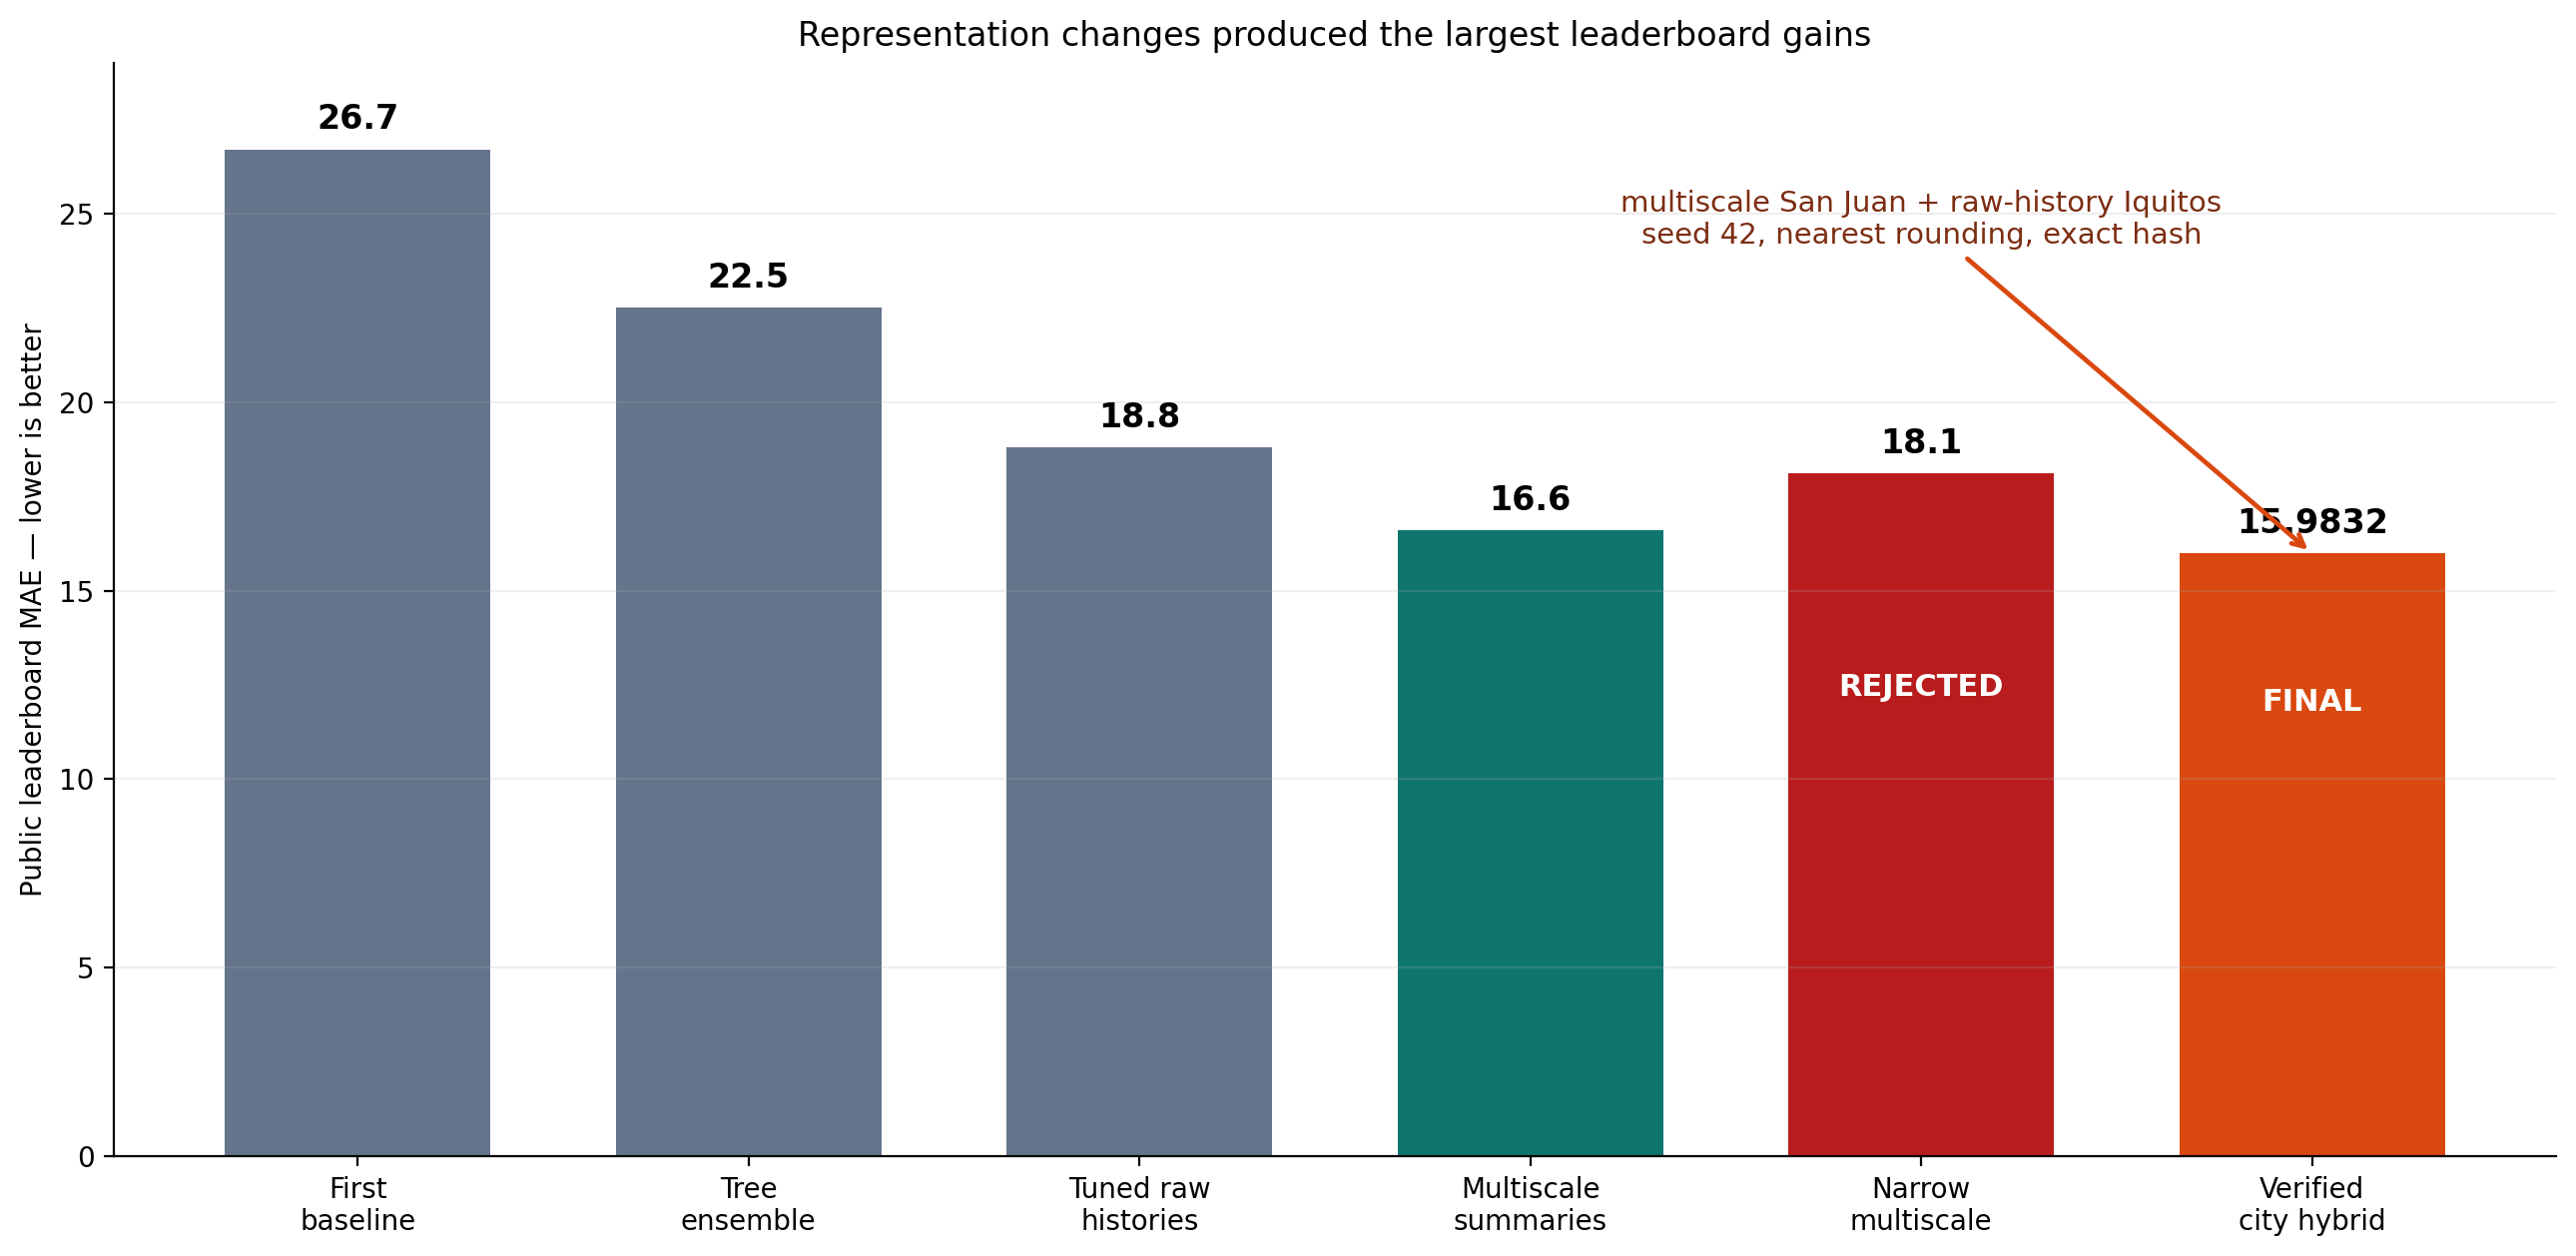
\includegraphics[width=0.9\linewidth]{figures/06_leaderboard_journey.png}
\caption{Observed public leaderboard MAE by stage. The final bar is the hash-verified city hybrid: multiscale San Juan, raw-history Iquitos and nearest-integer rounding.}
\label{fig:journey}
\end{figure}

\subsection{The rejected experiments were part of the result}
The score sequence can look deceptively direct in hindsight. In practice, much of the work was spent establishing what \emph{not} to trust. We preserved the most informative negative results in Table~\ref{tab:rejected}; they explain why the final system is a hybrid rather than the winner of one large hyperparameter search.

\begin{table}[H]
\centering
\caption{Experiments that did not enter the final submission and the information they contributed.}
\label{tab:rejected}
\small
\begin{tabular}{>{\raggedright\arraybackslash}p{4.0cm}>{\raggedright\arraybackslash}p{4.8cm}>{\raggedright\arraybackslash}p{5.4cm}}
\toprule
\textbf{Experiment} & \textbf{What happened} & \textbf{Lesson carried forward}\\
\midrule
XGBoost/CatBoost and forest blends & Better training/development behaviour and lower local MAE, but worse hidden generalisation & Temporal validation is evidence, not proof; preserve a simple fallback and check prediction amplitude\\
Forest hyperparameter and component search & Several mixtures won on development origins but not on the untouched recent origin & Prefer small, stable gains; use test-length chronological horizons\\
Negative-binomial, volatility, recency and quantile corrections & Plausible count/time-series ideas did not improve robustly enough to replace the confirmed forest & A sophisticated output model cannot recover climate history that is absent from the input\\
Three-seed raw-lag MLP ensemble & Averaging seeds scored $19.5$, while seed $42$ scored $18.8$ & Averaging highly correlated models can shrink rare peaks instead of adding useful diversity\\
Raw lags plus summaries & More inputs were worse than summaries alone ($18.43$ vs. $12.61$ in the two-fold ablation) & The gain was compression and inductive bias, not simply more information\\
Narrow $48\rightarrow12$ multiscale MLP & Won local architecture search by $0.224$ MAE but lost public leaderboard by $1.5$ MAE & Freeze the proven network when a searched local gain is smaller than fold variance\\
\bottomrule
\end{tabular}
\end{table}

This effort was worthwhile because each negative result narrowed the diagnosis. Model-family tuning exposed generalisation risk; peak-by-peak residual inspection exposed missing temporal context; the raw-plus-summary ablation provided
additional evidence that compact temporal
representations were more effective than
simply increasing the number of inputs
under the tested model configuration. The final score is therefore the end of an evidence chain, not a lucky architecture choice.

\subsection{Local validation is evidence, not proof}
After shrinking the input from $461$ to $180$, a local architecture search preferred a narrower $48\rightarrow12$ network by only $0.224$ validation MAE, and its outbreak error was already worse. On the public leaderboard it was $1.5$ MAE \emph{worse} ($18.1$ vs.\ $16.6$; Figure~\ref{fig:trap}). A small win after searching many candidates is likely selection noise. The representation survived public leaderboard testing; the architecture difference did not. We therefore froze the $100\rightarrow25$ San Juan network and concentrated on controlled ablations of the representation.

\begin{figure}[H]
\centering
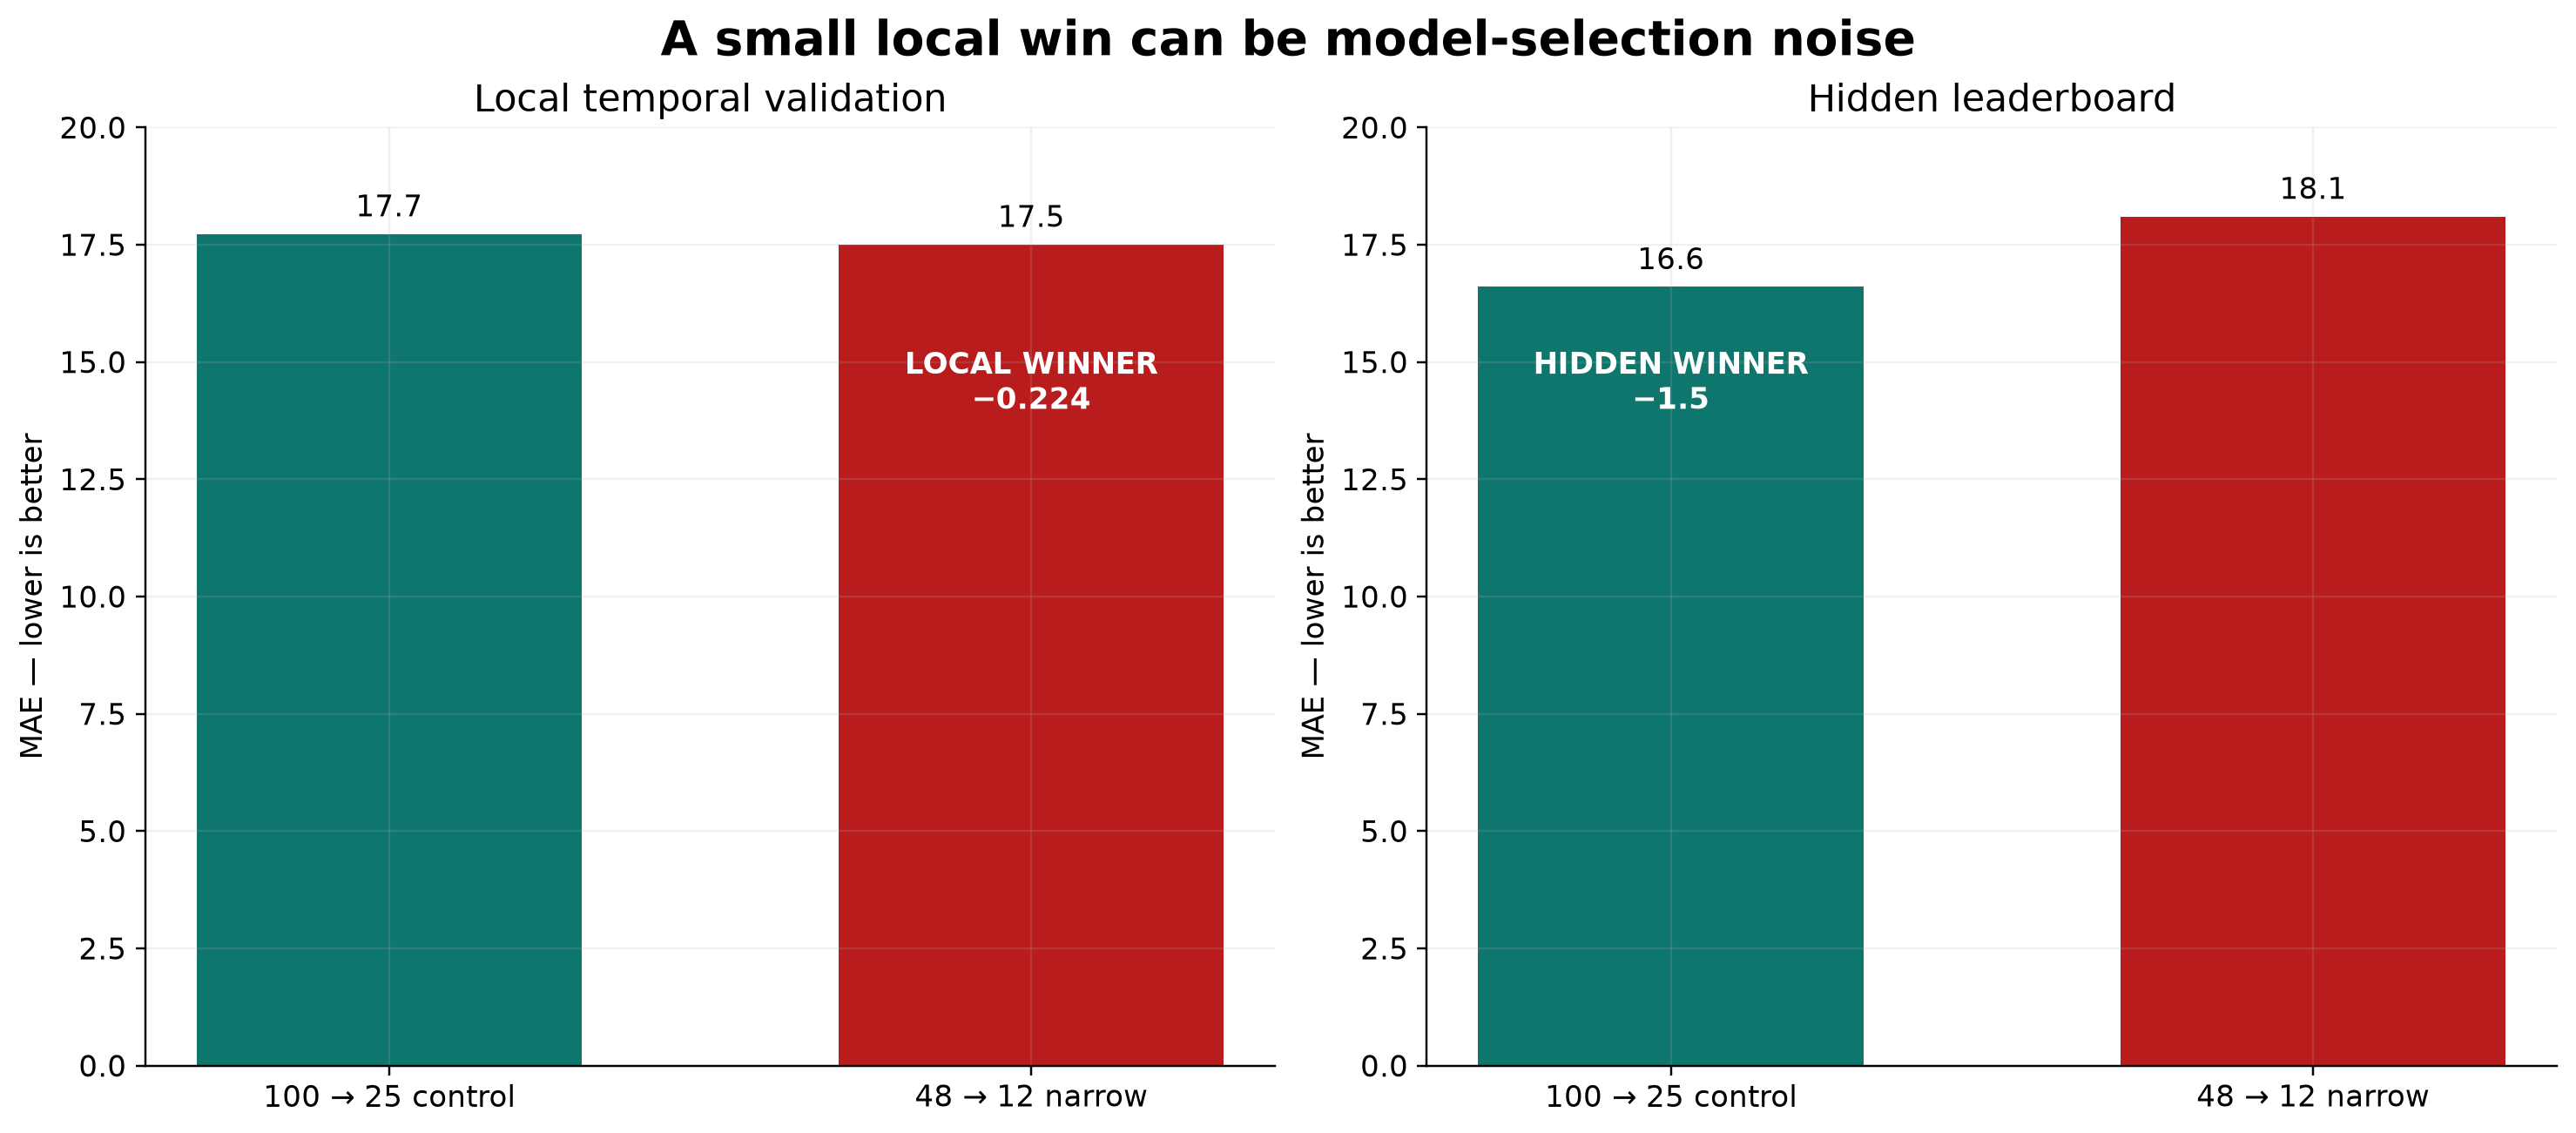
\includegraphics[width=0.9\linewidth]{figures/07_local_validation_trap.png}
\caption{The $48\rightarrow12$ network looked better locally ($-0.224$) but was worse on the public leaderboard ($+1.5$).}
\label{fig:trap}
\end{figure}

\subsection{Final submission and leaderboard performance}

The final submission combines city-specific
models with different temporal representations.

For San Juan, we use 180 multiscale climate
features. This representation is processed by
an MLP with hidden layers
of 100 and 25 units.

For Iquitos, we retain the tuned raw-history
MLP with 380 input features and hidden layers
of 70 and 18 units.

Both models generate non-negative integer
predictions, which are assembled according
to the official submission template. San Juan
uses nearest-integer rounding; Iquitos predictions
come from the preserved seed-$42$ raw-history file.

\begin{figure}[h]
    \centering
    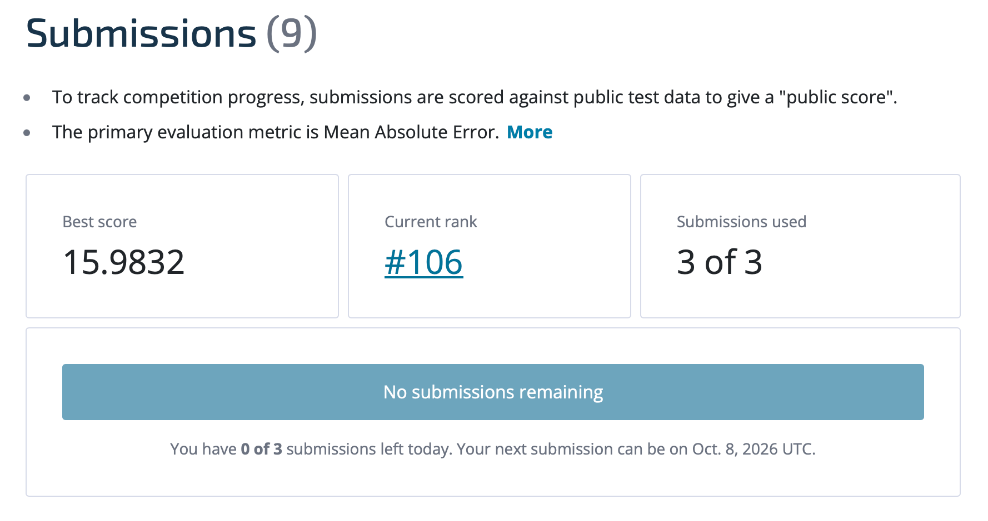
\includegraphics[
        width=0.8\linewidth
    ]{figures/submission_screenshot.png}

    \caption{
        Final DengAI public leaderboard result.
        The model achieved an MAE of 15.9832
        and was ranked 106th at the time of capture.
        This result is distinct from chronological
        cross-validation performance.
    }
    \label{fig:final_leaderboard}
\end{figure}
The final system achieved a public
leaderboard MAE of \textbf{15.9832},
with a rank of \textbf{106} at the time
of evaluation, as shown in
Figure~\ref{fig:final_leaderboard}.

This result provides evidence of performance
on the competition's public evaluation period.
However, it does not independently establish
generalization to unseen cities or future
epidemic periods.

Detailed implementation instructions,
experimental configurations, and source code
are provided in our GitHub repository.

The reproduction notebook recreated all $416$
predictions exactly. Both the restored and generated
files have the following SHA-256:
\par\noindent
\submissionhash.



% Nearest-integer rounding details are reported in Section~\ref{sec:finalrecipe}.

% \begin{figure}[H]
% \centering
% 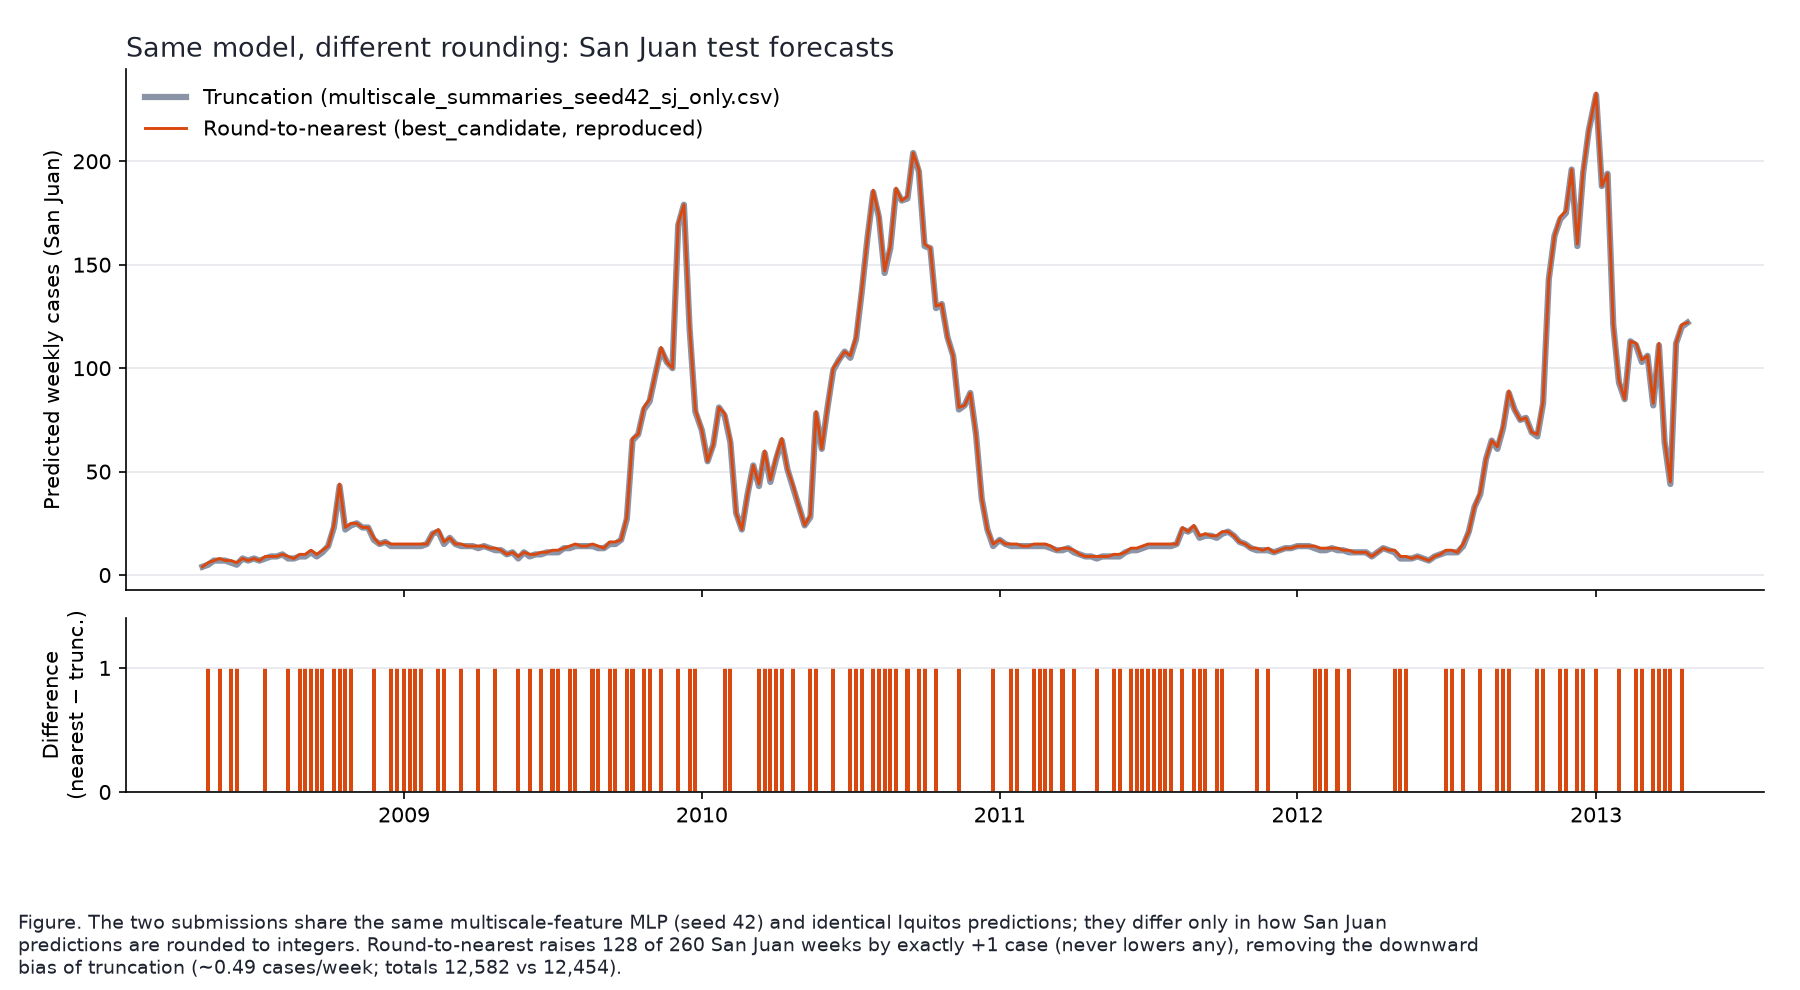
\includegraphics[width=\linewidth]{figures/rounding_comparison.png}
% \caption{San Juan test forecasts of the final model with truncation vs.\ round-to-nearest (top) and their difference (bottom).}
% \label{fig:rounding}
% \end{figure}

\subsection{Error analysis}
\begin{itemize}
  \item \textbf{Outbreaks changed the representation.} In San Juan the outbreak-week MAE ($\approx 56$) is more than three times the mean MAE ($\approx 18$) (Table~\ref{tab:repr}). The early trees predicted the seasonal envelope but missed abrupt peaks whose same-week weather looked ordinary. That residual pattern, not a generic desire for more features, motivated delayed climate windows and then multiscale summaries. The final model times major rises more convincingly, although peak amplitude remains uncertain.
  \item \textbf{Fold variance is large.} The worst San Juan fold ($27.3$) is much worse than the mean ($17.7$): performance depends on which year is held out.
  \item \textbf{Single seeds mislead.} The $18.8$ result had a three-seed mean of $19.5$.
  \item \textbf{Iquitos is near its floor.} Climatology is as good as complex models on Iquitos validation weeks ($\approx 7$), consistent with its small, noisy counts.
\end{itemize}


\section{Discussion}

\subsection{Feature engineering as the primary driver of performance}

The central finding of this project is that the representation
of climate history played a more important role in our
experiments than increasing model complexity.
Rather than continuously introducing more sophisticated
predictive models, our largest improvements came from
investigating what information the models received
and how that information was represented.

\paragraph{From instantaneous observations to temporal history.}

Our initial tree-based models used current climate
measurements, selected lags, rolling statistics, and
seasonal features. Although these models captured
general seasonal patterns, error analysis revealed
that they frequently underestimated large dengue
outbreaks.

This observation motivated us to investigate delayed
relationships between climate conditions and dengue
incidence. We constructed city- and variable-specific
history windows, producing 461 input coordinates for
San Juan and 380 for Iquitos.

The raw-history MLP improved the public leaderboard
MAE from 22.5 to 18.8 after temporal and architectural
tuning. This result suggested that richer historical
climate information could be useful for prediction.
However, because both the model family and feature
representation changed, this improvement cannot be
attributed exclusively to feature engineering.

\paragraph{From raw histories to multiscale representations.}

Although raw histories preserve detailed temporal
information, they also introduce hundreds of highly
correlated inputs. This creates an inefficient
representation for a dataset containing only
936 San Juan and 520 Iquitos training observations.

We addressed this limitation by constructing 11
statistics for each of the 16 weather variables,
together with four cyclic seasonal features,
resulting in 180-dimensional input vectors.

These features represent climate conditions at
multiple timescales, including current levels,
short- and long-term averages, variability,
recent changes, and temporal trends.

Importantly, the multiscale representation
does not merely reduce dimensionality.
It introduces an inductive bias by explicitly
providing temporal patterns that the MLP would
otherwise need to learn from individual weekly
observations.

Under the same tuned MLP and chronological
validation procedure, the multiscale
representation reduced the mean MAE in San Juan
from 20.635 to 17.726 and in Iquitos from
7.908 to 7.588.

The public leaderboard MAE also improved
from 18.8 to 16.6.

These controlled experiments provide our
strongest evidence that temporal feature
representation was a major contributor
to predictive performance.

\paragraph{Why adding more features was not sufficient.}

We additionally compared raw histories,
multiscale summaries, and their concatenation.

The combined representation performed worse
than the multiscale representation alone
in the reported two-fold ablation.

This finding suggests that useful feature
engineering is not simply the addition of
more information or input dimensions.

Instead, constructing compact and meaningful
representations can improve the inductive bias
and optimization behavior of neural networks
trained on relatively small datasets.

Nevertheless, this experiment does not
independently isolate dimensionality reduction
from changes in optimization and regularization.

\paragraph{Artifact recovery changed the conclusion.}

The final CSV is part of the experimental evidence,
not merely an export. Recovering it allowed us to
match every prediction to its recorded recipe and
correct a mistaken PLS attribution. The notebook
also showed that the numerical environment is part
of the model: Python $3.12$ with NumPy $2.4.4$
reproduced the artifact exactly, whereas an older
NumPy environment did not. For small neural models,
code, data, package versions, output file and hash
must therefore be archived together.

\subsection{Limitations and implications}

Despite these improvements, dengue prediction
remains challenging, particularly during rare
and extreme outbreaks.

Our experiments showed that lower overall MAE
does not necessarily imply better prediction
of outbreak weeks. In Iquitos, for example,
multiscale summaries slightly increased
outbreak-week MAE despite improving average
validation performance.

Furthermore, our results are limited to two
cities, a relatively small historical dataset,
and the climate measurements supplied by the
competition.

The historical feature-construction pipeline
also contains alignment and temporal-context
behaviors that require further causal auditing
before prospective forecasting claims can
be established.

Therefore, the observed leaderboard performance
should not be interpreted as direct evidence of
real-world early-warning effectiveness.

\paragraph{Main lesson.}

Our findings emphasize that, particularly for
small time-series datasets, the quality and
structure of input features can be as important
as the choice of predictive algorithm.

In our experiments, the most convincing
improvements emerged from diagnosing missing
temporal information, constructing multiscale
summaries, and preserving a city-specific hybrid.

The broader lesson is that feature engineering
should be treated as a central part of model
design rather than merely a preprocessing step.


\section{Future work}
\label{sec:future}
\begin{itemize}
  \item Repeat the multiscale MLP over more temporal cut points and seeds, and archive each exact submitted CSV, manifest and hash alongside its score.
  \item Evaluate PLS prospectively as a separate leakage-safe experiment rather than attributing it to the existing $15.9832$ artifact.
  \item Quantify uncertainty (quantile loss or ensembles over seeds) to give outbreak risk bands rather than a single count.
  \item Evaluate more folds and repeated seeds before accepting architecture changes smaller than the fold-to-fold spread.
  \item Test the representation on other cities or other vector-borne diseases.
\end{itemize}

\section{Conclusion}
This project investigated weekly dengue case prediction for San Juan and Iquitos using climate and vegetation measurements. Rather than treating model selection as the primary challenge, we progressively examined how temporal dependencies, feature representations, and model complexity influence predictive performance.

Our experiments produced three main findings. First, a model with better chronological validation performance did not necessarily achieve a better public leaderboard result, demonstrating the limitations of selecting models using a small number of temporal folds. Second, representing climate history through multiscale statistical summaries improved the performance of a fixed MLP architecture compared with raw lagged inputs. Third, the strongest submission was a city-specific hybrid rather than a single universal representation: San Juan used multiscale summaries and nearest rounding, while Iquitos retained its raw-history model.

The final hybrid system achieved a public leaderboard MAE of \textbf{15.9832}. Its $416$ predictions were reproduced exactly with a pinned environment and verified by SHA-256. Nevertheless, outbreak prediction remains difficult, and the benchmark does not directly establish prospective forecasting performance. Future work should examine strictly causal preprocessing, repeated-seed stability, and evaluation under realistic information-availability constraints.

Overall, the project highlights the importance of diagnosing model errors and designing informative temporal representations, rather than relying exclusively on increasingly complex predictive architectures.
%--------------------------------------------------------------------
\section*{Author Contributions}
%--------------------------------------------------------------------
\begin{itemize}
  \item \textbf{Duy Chien Nguyen:} Conducted data preprocessing, developed the baseline models, investigated Partial Least Squares (PLS) as a later representation experiment, made the presentation slides, and wrote the report.
  \item \textbf{Dang Quy Nguyen:} Conducted data preprocessing, developed and improved the tree-based methodologies, led feature engineering efforts, built the lagged feature representations and the Multi-Layer Perceptron (MLP) architecture,  made the presentation slides, and wrote the report.
\end{itemize}

%--------------------------------------------------------------------
\section*{Code Availability}

\begin{itemize}
  \item Data: DengAI training/test CSV files from the competition site.
  \item \textbf{Code Repository:} The complete source code, trained models, and reproducible notebooks are available on GitHub at \url{https://github.com/dangnq2501/DengAI}.
  \item \textbf{Presentation Video:} A recorded video of our project presentation can be viewed at \url{https://youtu.be/Et3oHyoi_VI}.
  \item The public leaderboard MAE $15.9832$ is a leaderboard observation associated with the restored artifact; hidden labels are unavailable locally.
  \item Reproduction generated the same $416$ predictions. Its SHA-256 is:\newline
  \submissionhash.
\end{itemize}

\begin{thebibliography}{9}
\bibitem{drivendata} DrivenData. \emph{DengAI: Predicting Disease Spread}. \url{https://www.drivendata.org/competitions/44/dengai-predicting-disease-spread/}
\bibitem{xgboost} T.~Chen and C.~Guestrin. XGBoost: A scalable tree boosting system. \emph{KDD}, 2016.
\bibitem{catboost} L.~Prokhorenkova et al. CatBoost: unbiased boosting with categorical features. \emph{NeurIPS}, 2018.
\bibitem{rf} L.~Breiman. Random forests. \emph{Machine Learning}, 45(1):5--32, 2001.
\bibitem{extratrees} P.~Geurts, D.~Ernst and L.~Wehenkel. Extremely randomized trees. \emph{Machine Learning}, 63(1):3--42, 2006.
\bibitem{selu} G.~Klambauer et al. Self-normalizing neural networks. \emph{NeurIPS}, 2017.
\bibitem{pls} S.~Wold, M.~Sj\"ostr\"om and L.~Eriksson. PLS-regression: a basic tool of chemometrics. \emph{Chemometrics and Intelligent Laboratory Systems}, 58(2):109--130, 2001.
\end{thebibliography}

\end{document}
